\chapter{Analysis}
     Here we present several comparisons of the data processed according to Chapter 2 vs. the AME properties determined in PCXV.  We describe an estimation of the FIR-emitting dust optical depth abundance vs. the spinning dust amplitude $A_{sp}$. From PCXV, $A_{sp}$ is \textit{``essentially the flux density at the peak normalized to the spinning dust model."}.  We also include a look at each waveband's averaged intensity described in Chapter 2, for each of the 98 ROIs, vs. the $A_{sp}$. This band-by-band fitting is repeated with the average intensities scaled by interstellar radiation field strength (ISRF) of each ROI (the ISRF is given as $G0$, which is the ISRF strength compared to that of the solar neighborhood). Lastly, we revisit an earlier result of the 9 to 18~$\mu$m ratio vs. the significance of the spinning dust model fit for each ROI. Our previous result included only 10 ROIs from PCXV, the present result includes all 98.

\section{Dust Optical Depth vs. AME Amplitude}
     After color-correction and obtaining a fitted value the temperature, $T$ and optical depth at 250~$\mu$m, $\tau_{250}$. of each pixel, we estimate the relative total far infrared emission (FIR) at each pixel using the following equation, where $\lambda$ is the wavelength in microns, $\tau_{250}$ is the optical depth at 250~$\mu$m, and $B(T)$ is the Planck function:

\begin{equation}
\label{FIR}
FIR = \tau_{250\mu m} \int_{0}^{\infty} [250\mu m/\lambda(\mu m)]^{\beta}
B_{\lambda}(T) d\lambda ,\;
%\label{totalFIR}
\end{equation}
%To explain further, we must carefully introduce a conventional term, "sub-micron dust". This term does not cover all of the dust which is smaller than one micron. PAH carriers and VSGs are not included in "sub-micron dust". Instead, this term refers to grains which are large enough to emit in a classical way (modified blackbody), but are not larger than one micron. 
     The total FIR emission derived above is a result of the incident radiation on the dust (essentially, the incoming starlight) and the column density of the FIR-emitting dust. This property of dust emission is well-described in \cite{onaka00}. For our analysis we use $\tau_{250\mu m}$ as a tracer of the FIR-emitting, or ``classically emitting" dust, This is because $\tau_{250\mu m}$ is proportional to the column density of FIR-emitting dust; FIR emission at 250~$\mu m$ should be dominated by the modified blackbody emission from such grains. The FIR emission does not include very small grains or PAH-type molecules. 
     For the present analysis, we use a version of the modified blackbody fitting where $\beta$ is fixed at 2. The issue of the most appropriate treatment of $\beta$ will be revisited in a future investigation, where we allow beta to vary.
     The above calculation is carried out for each of the 98 candidate regions, and plotted against $A_{sp}$. Figures 3.1 and 3.2 show resulting plot for the regions with high AME significance and regions of low AME significance, respectively. While our comparisons with the PCXV AME parameters uses only the averaged results of the modified blackbody fitting, we have included the pixel-by-pixel results as well in Appendix A. There you can see each region's structure in terms of $T$, $\tau_{250}$, $G0$, and reduced $\chi^2$. Appendix B shows the average SED plots of each region: the averaged observed intensity at each waveband overplotted with the region's average modified blackbody curve.

%We also show the results using a slightly different comparison. Instead of $A_{sp}$, we use the ``residual flux" of each ROI in the 28.4 GHz Planck LFI band. Since we have not done our own modelling of the spinning dust spectrum, we felt it is best to include also a more robust comparison with the AME. A comparison of the IR bands with the residual 28.4 GHz flux is independent of a spinning dust explanation. However in order to compare them directly, we first convert our data to flux density units by multiplying by the solid angle of each region. The solid angle is obtained from the count of the unmasked pixels for each ROI, multiplied by the solid angle per pixel. One potential issue however is that in order to determine the AME flux density, thermal dust must be subtracted. The Planck Collaboration subtraction of thermal dust from the LFI data is based on the HFI data. If this subtraction is not complete (i.e. the residual AME flux is not entirely residual), it may complicate the situation since we are attempting to compare the thermal dust information vs. the AME.
     
\subsection{Non-Significant AME Regions}
     To investigate if there is a difference in the correlation of sub-micron dust relative abundance in regions well-modelled by a spinning dust spectrum vs. those that are not, we separate the ROIs into two subsamples. Figure 3.2 shows that there is still a correlation with $A_{sp}$ for the low AME significance regions ($\sigma AME < 5$). However the correlation is slightly weaker than with the regions that are fitted nicely by the spinning dust model ($\sigma AME > 5$).      
\begin{figure}[!htbp]
\begin{center}
\label{fig:tauvsaspnosp}
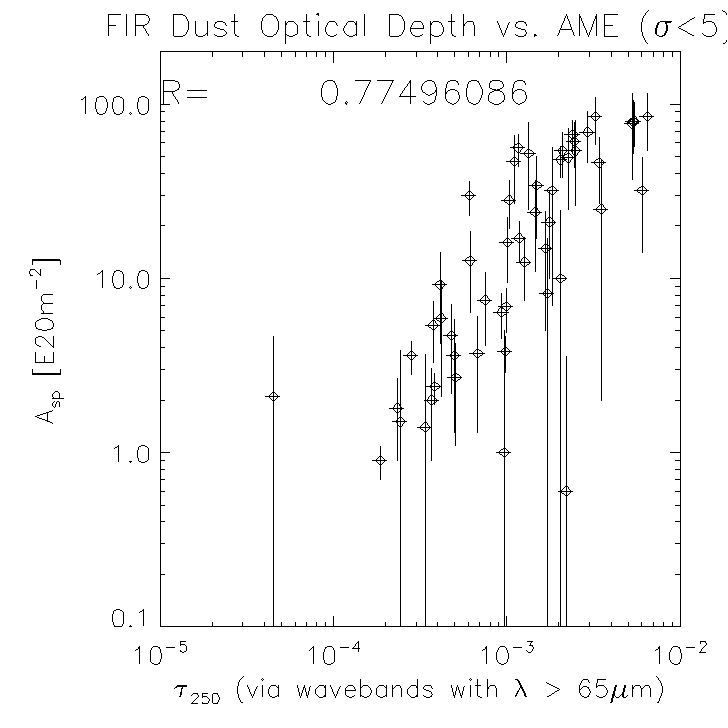
\includegraphics[width=150mm]{EPS/tau250vsAspnosp_masterpres.pdf}
  \caption{ This figure shows only the regions having an AME significance below 5$\sigma$. The correlation coefficient R is 0.77. These regions are classified as ``non-significant AME regions" in \cite{planckXV}. The error bars here are larger by definition, since $\sigma AME$ is given by PCXV as the S/N ratio of $A_{sp}$.}
\label{sub-micron dust vs. Spinning dust}
\end{center}
\end{figure}

\subsection{AME Regions}
     Finally, regions that PCXV found to be well-fitted by the spinning dust model are plotted as a subsample (see Figure \ref{fig:tauvsaspsp}). These regions all have a $\sigma$AME value $>$ 5. The subsample size is smaller than that of the non-significant AME regions (Figure 3.1). Again we can note a correlation, and that it is marginally stronger than the correlation using non-significant AME regions. We expect the correlation in Figure 3.2 to be the stronger one, assuming dust carries the AME.
\begin{figure}[!htbp]
\begin{center}
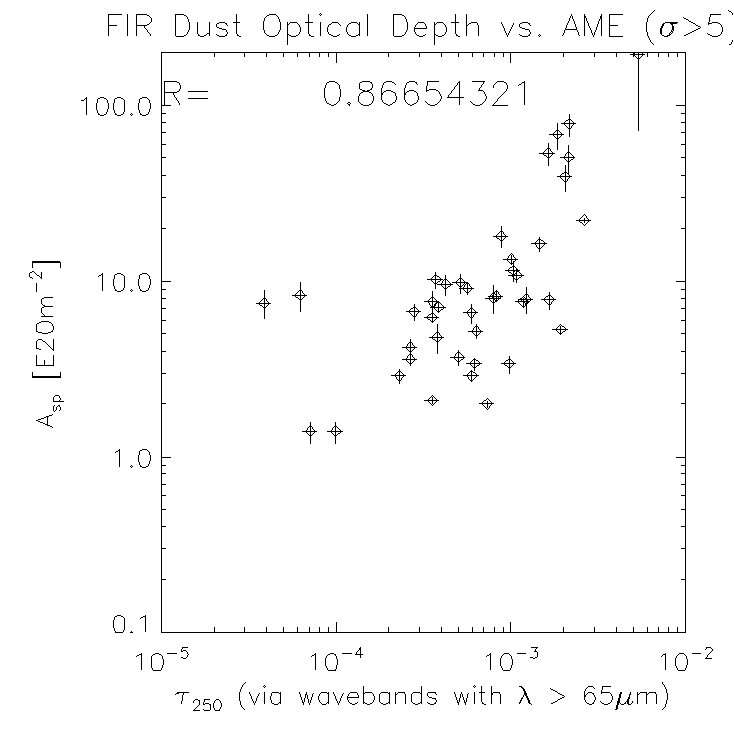
\includegraphics[width=150mm]{EPS/tau250vsAspsp_masterpres.pdf}
  \caption{The counterpart to Figure 3.1, this plot shows $A_{sp}$ vs. the relative sub-micron dust abundance for significant AME regions. The correlation coefficient R is 0.87. These regions have $\sigma$ AME $\>$ 5. This plot shows a slightly stronger trend than the plot of non-significant AME regions}
\label{fig:tauvsaspsp}
\end{center}
\end{figure}     
     
\section{Band-by-band Comparison against AME Amplitude}
     We perform a simple comparison of the averaged IR intensity vs. the spinning dust amplitude (PCXV) of each of the 98 ROIs. Our objective is to explore the possibility of a link between specific dust populations, such as PAHs, and the AME. As described in the introduction, such efforts have already been made by PCXV, \cite{leitch98}, and \cite{ysard10a} with respect to the IRAS all-sky maps. Looking at the individual bands' photometry, especially at the MIR bands, is important because MIR emission which seems in excess of the sub-micron dust abundance is thought to trace very small grains (VSG) or PAHs. 
     We present for the first time an AME vs. IR comparison via AKARI/IRC and FIS in Figures \ref{fig:IRIntMWAmpsp} and \ref{fig:IRIntMWAmpnosp}. These are shown along with the previously investigated IRAS bands. Additionally, we have utilized the HFI bands at 857~GHz and 545~GHz in order to constrain the long wavelength tail of the FIR thermal emission. We compare the relative strengths of the correlations across all 13 bands. As further analysis, Figures \ref{fig:IRIntG0MWAmpsp} and \ref{fig:IRIntG0MWAmpnosp} show how the results change when the IR intensity is scaled by the ISRF strength, $G0$.

\subsection{Average Infrared Intensity $I({\lambda})$ vs. AME Amplitude $A_{sp}$}
Figure \ref{fig:IRIntMWAmpsp} shows each waveband's averaged intensity for each ROI against the AME amplitude, $A_{sp}$, of each region. At least a weak covariance is seen for all bands.

\begin{figure}[!htb]
\centering
 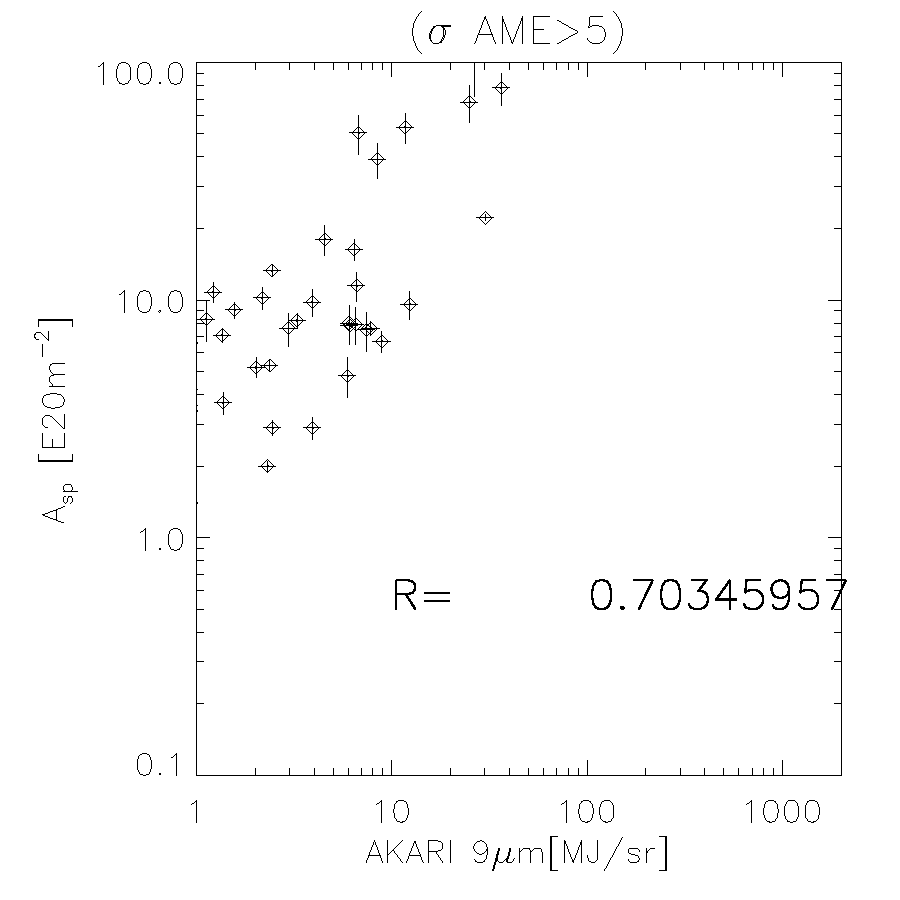
\includegraphics[width=50mm]{IRIntMWAmp/akari9_Asp_sp.pdf}
  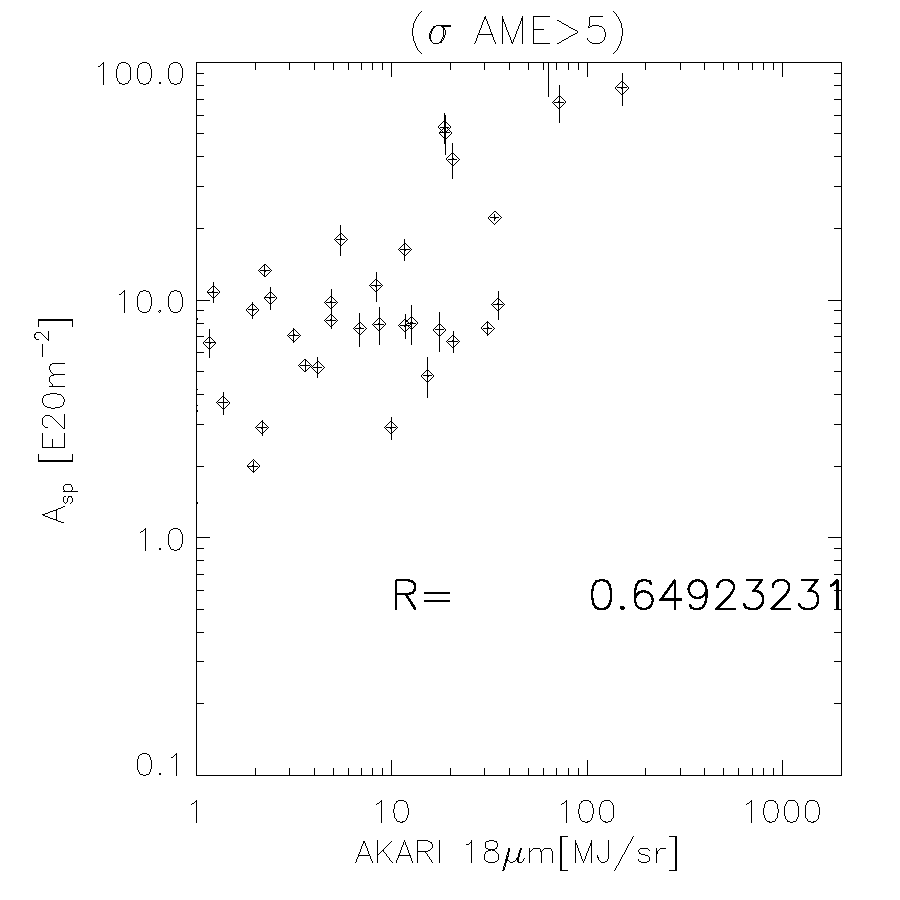
\includegraphics[width=50mm]{IRIntMWAmp/akari18_Asp_sp.pdf}
  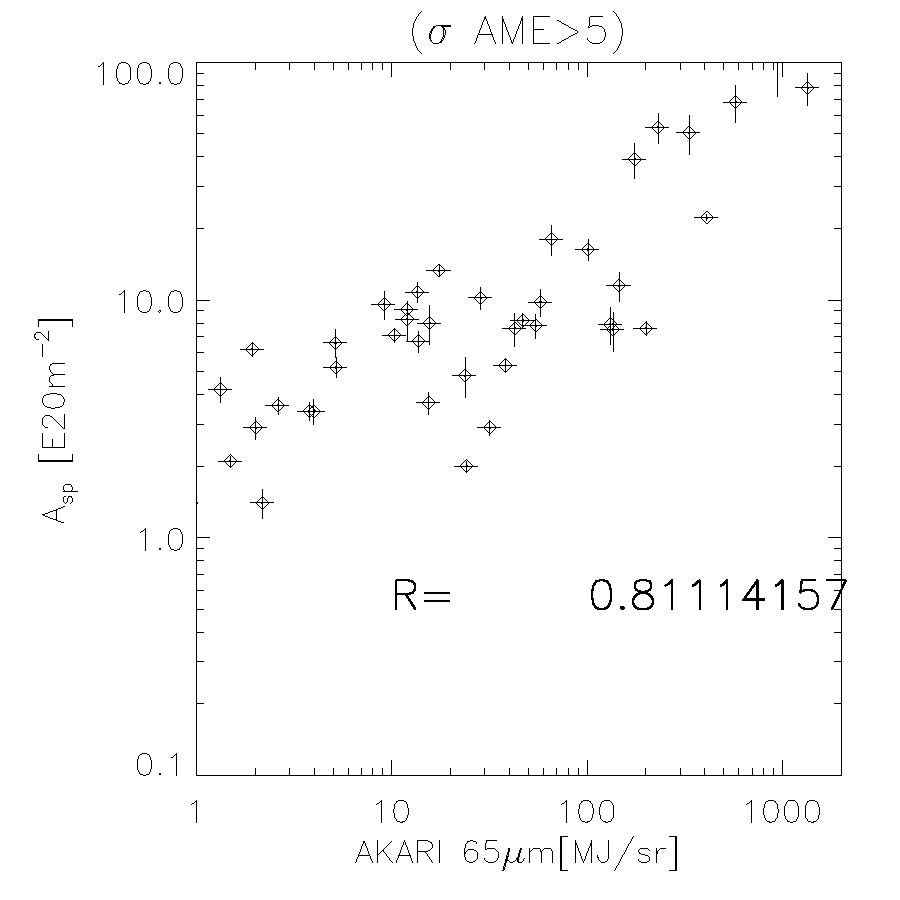
\includegraphics[width=50mm]{IRIntMWAmp/akari65_Asp_sp.pdf}
  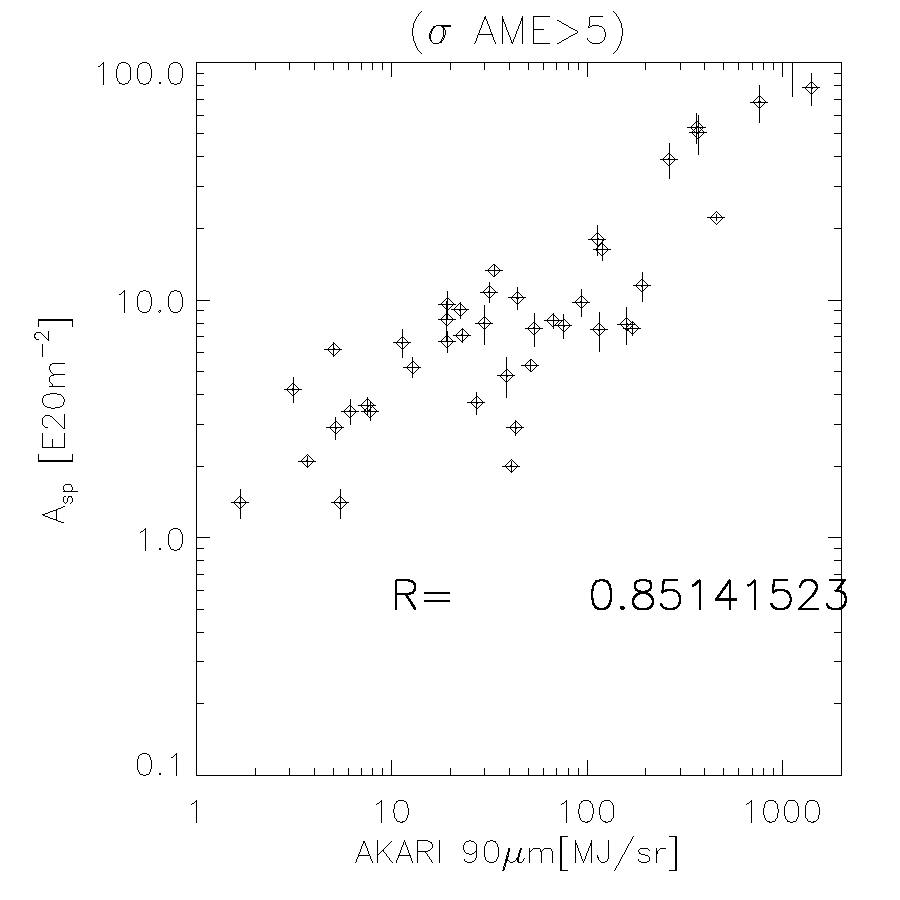
\includegraphics[width=50mm]{IRIntMWAmp/akari90_Asp_sp.pdf}
  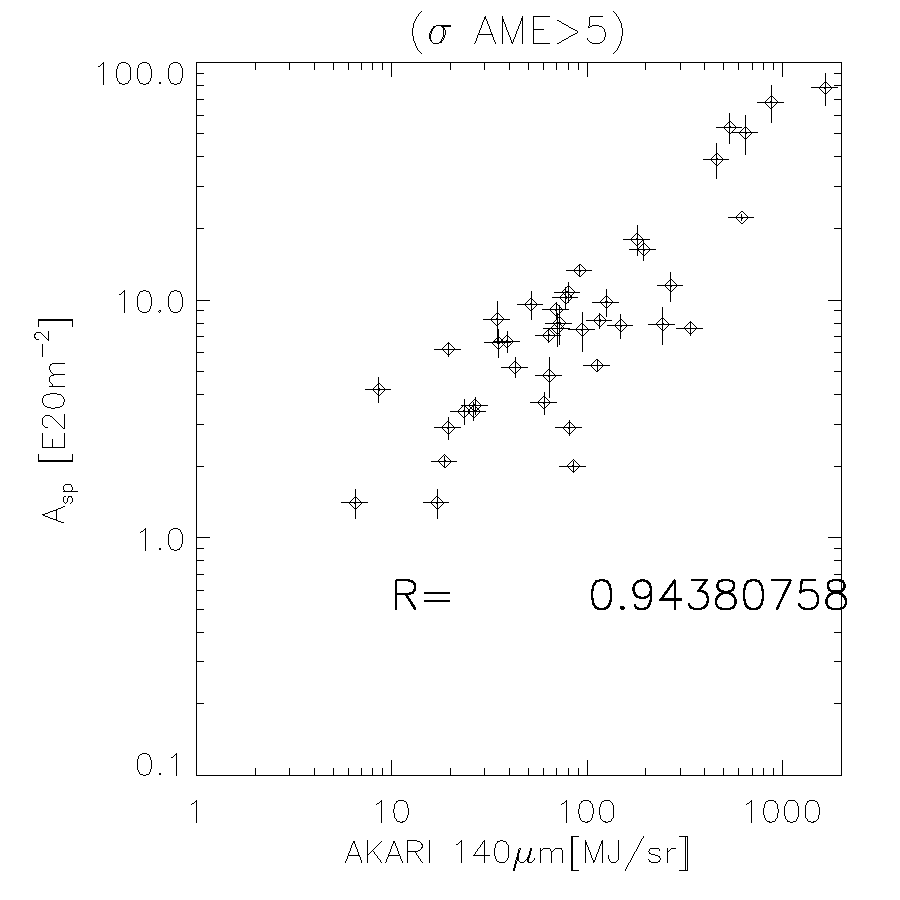
\includegraphics[width=50mm]{IRIntMWAmp/akari140_Asp_sp.pdf}
  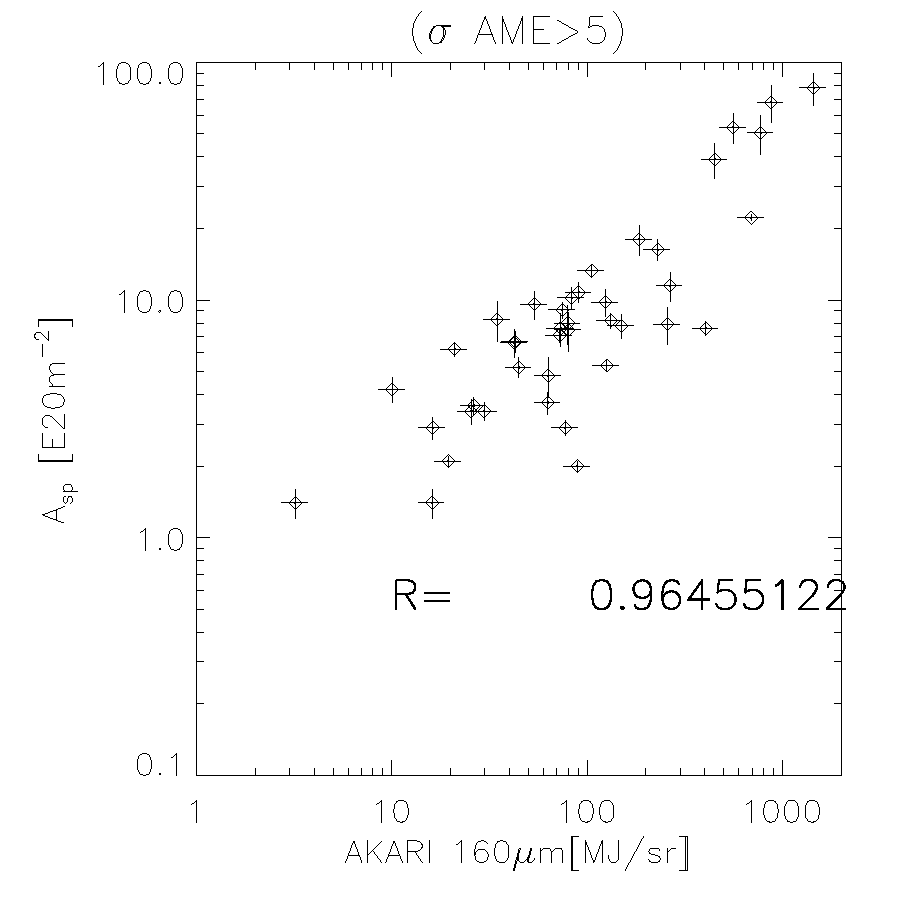
\includegraphics[width=50mm]{IRIntMWAmp/akari160_Asp_sp.pdf}
  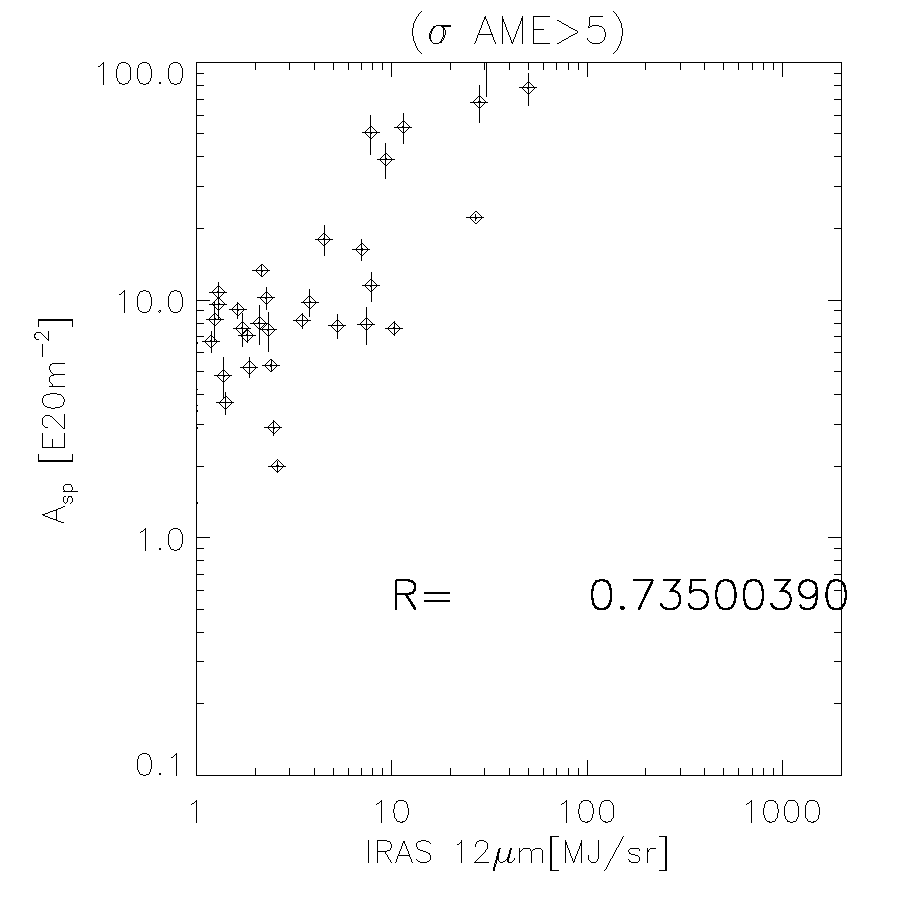
\includegraphics[width=50mm]{IRIntMWAmp/iras12_Asp_sp.pdf}
  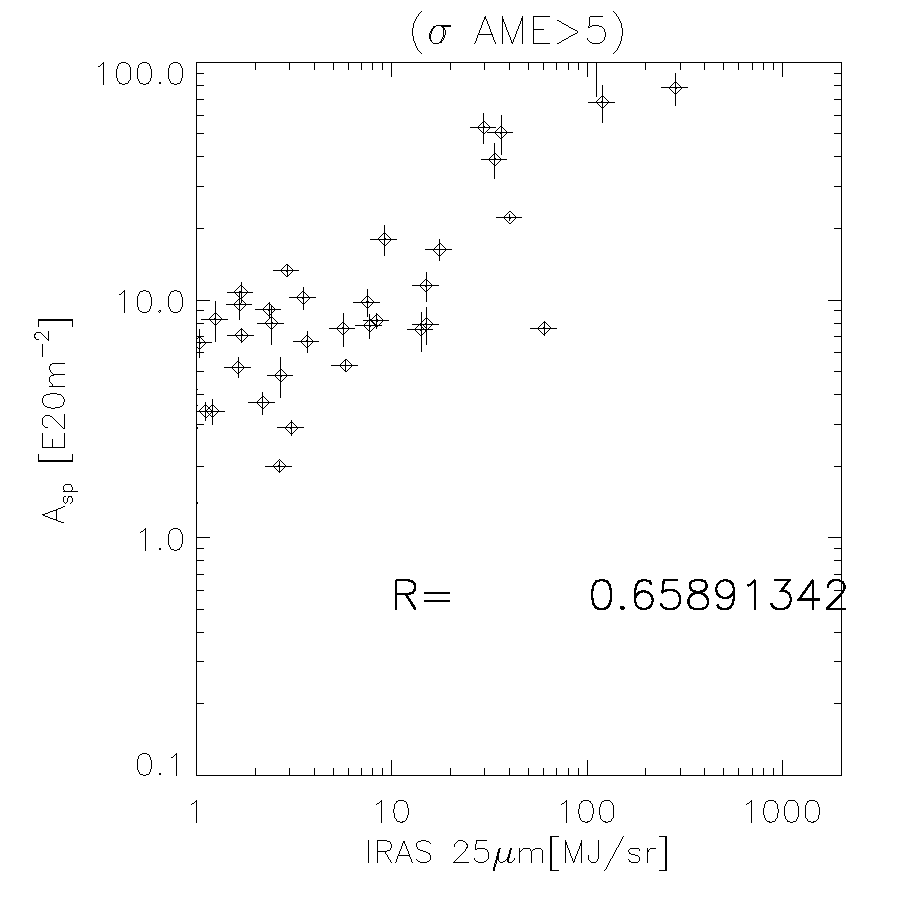
\includegraphics[width=50mm]{IRIntMWAmp/iras25_Asp_sp.pdf}
  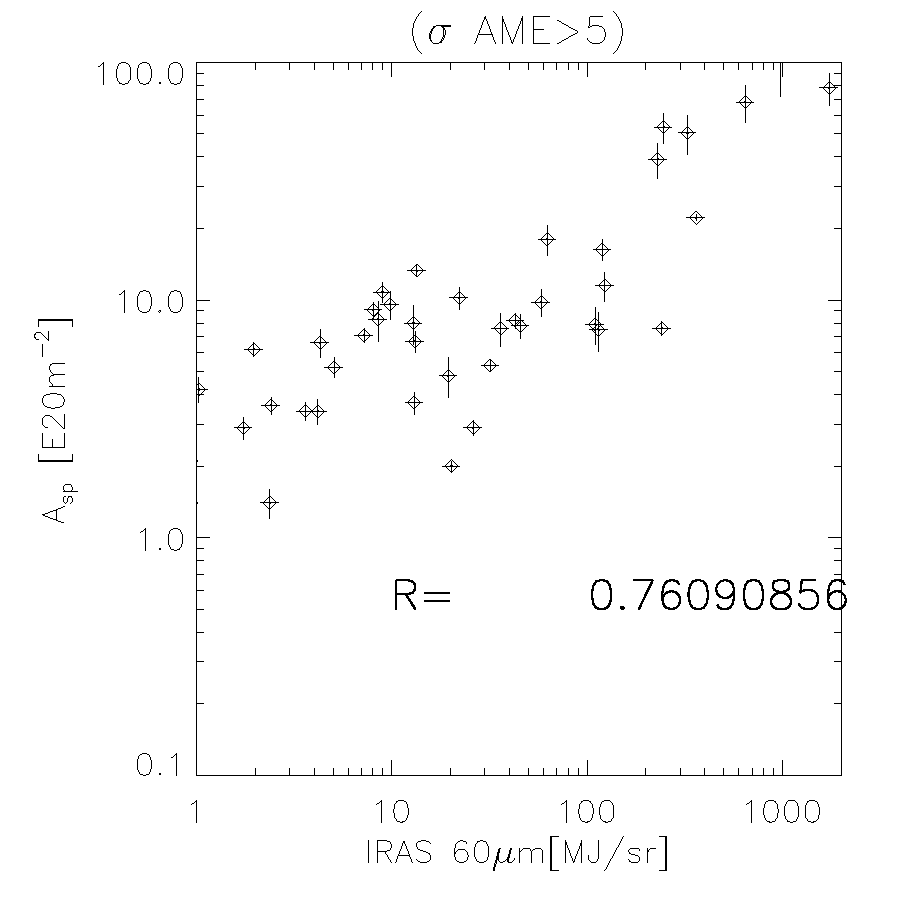
\includegraphics[width=50mm]{IRIntMWAmp/iras60_Asp_sp.pdf}
  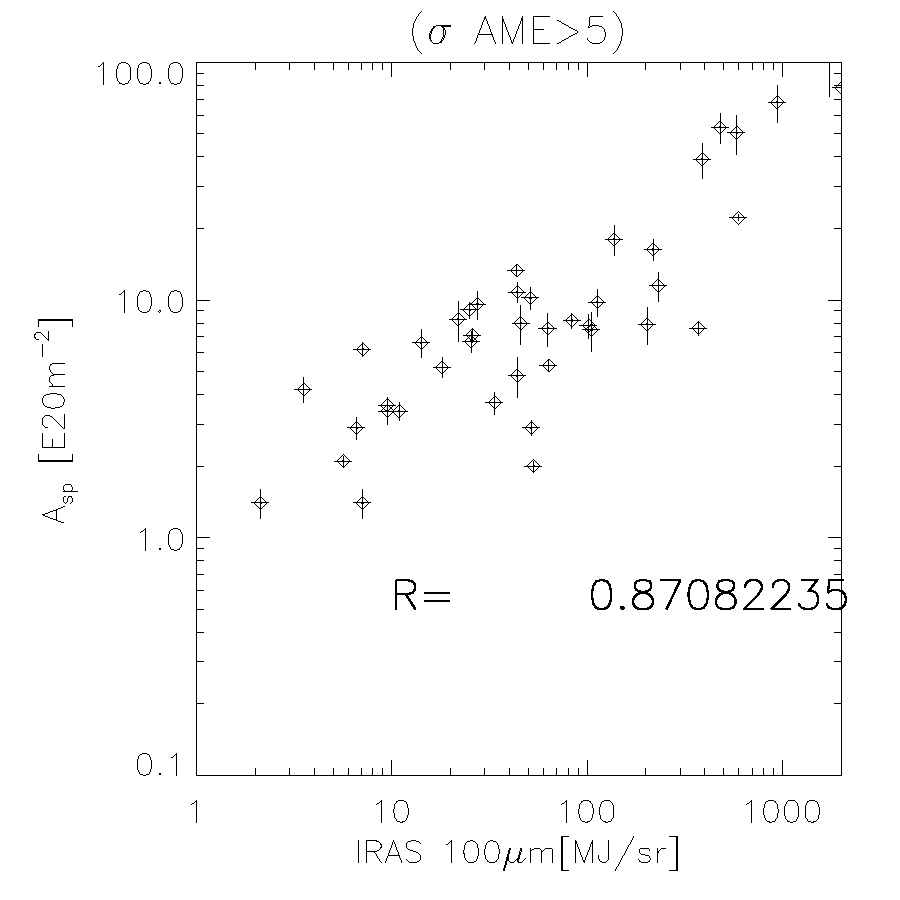
\includegraphics[width=50mm]{IRIntMWAmp/iras100_Asp_sp.pdf}
  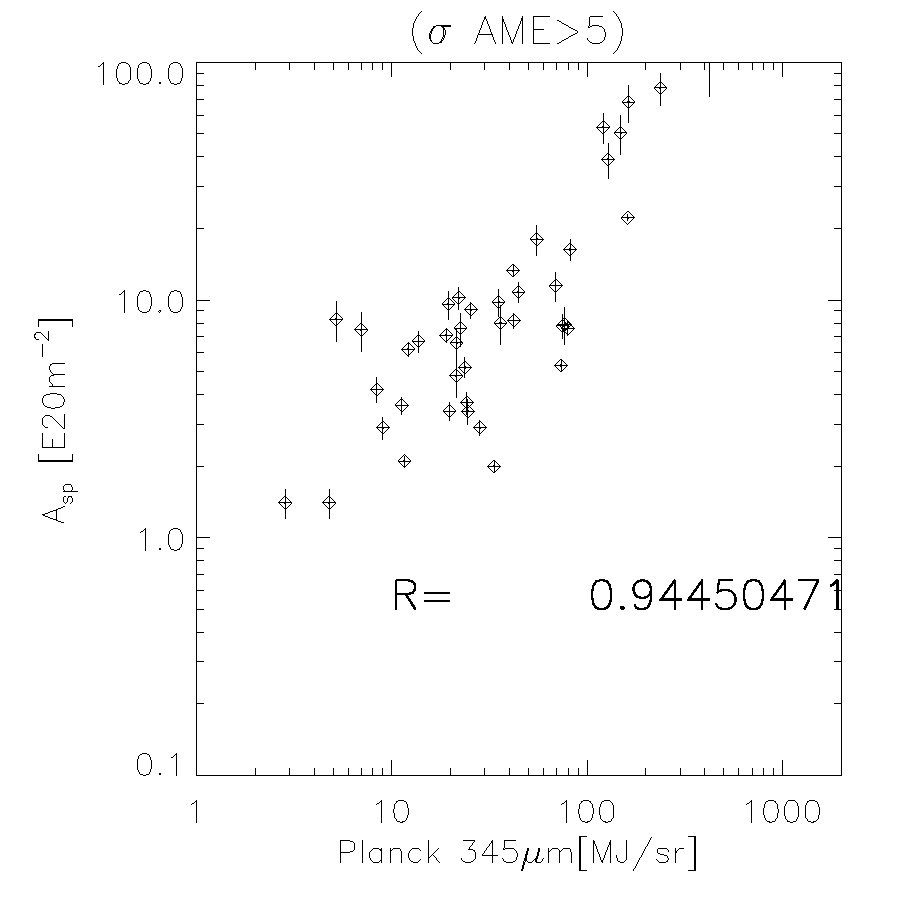
\includegraphics[width=50mm]{IRIntMWAmp/planck857_Asp_sp.pdf}
  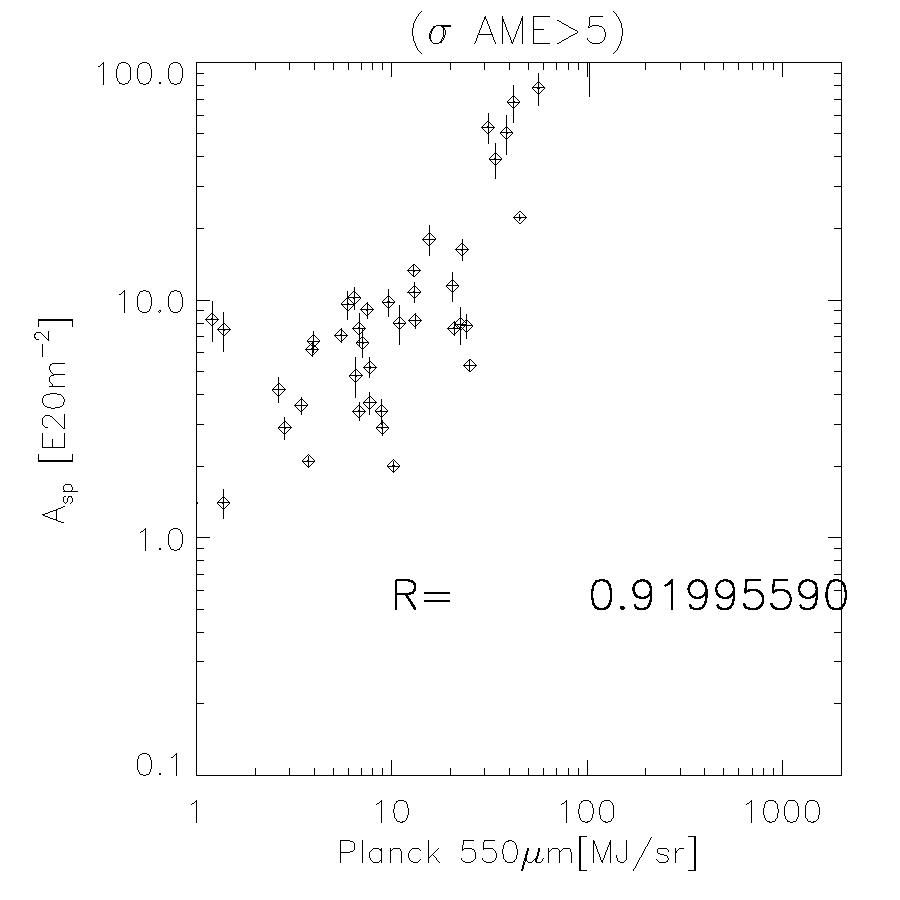
\includegraphics[width=50mm]{IRIntMWAmp/planck545_Asp_sp.pdf}
\caption{AME Amplitude vs. Infrared Photometry: Shown above for each waveband used in the analysis (from AKARI/IRC 9~$\mu$m to Planck/HFI 550~$\mu$m) are the average infrared intensities of each AME region from PCXV against each region's $A_{sp}$ value. These figures are roughly comparable to Figures \ref{planckcorrel} and \ref{ysardcorrel} from \cite{planckXV} and \cite{ysard10a}, respectively. A tighter fit to the AKARI 9~$\mu$m and other MIR bands (stochastically emitting dust) vs. that of $\tau_{250}$ (classically emitting dust), is not seen.
}
\label{fig:IRIntMWAmpsp}
\end{figure}
\begin{figure}[!htb]
\centering
 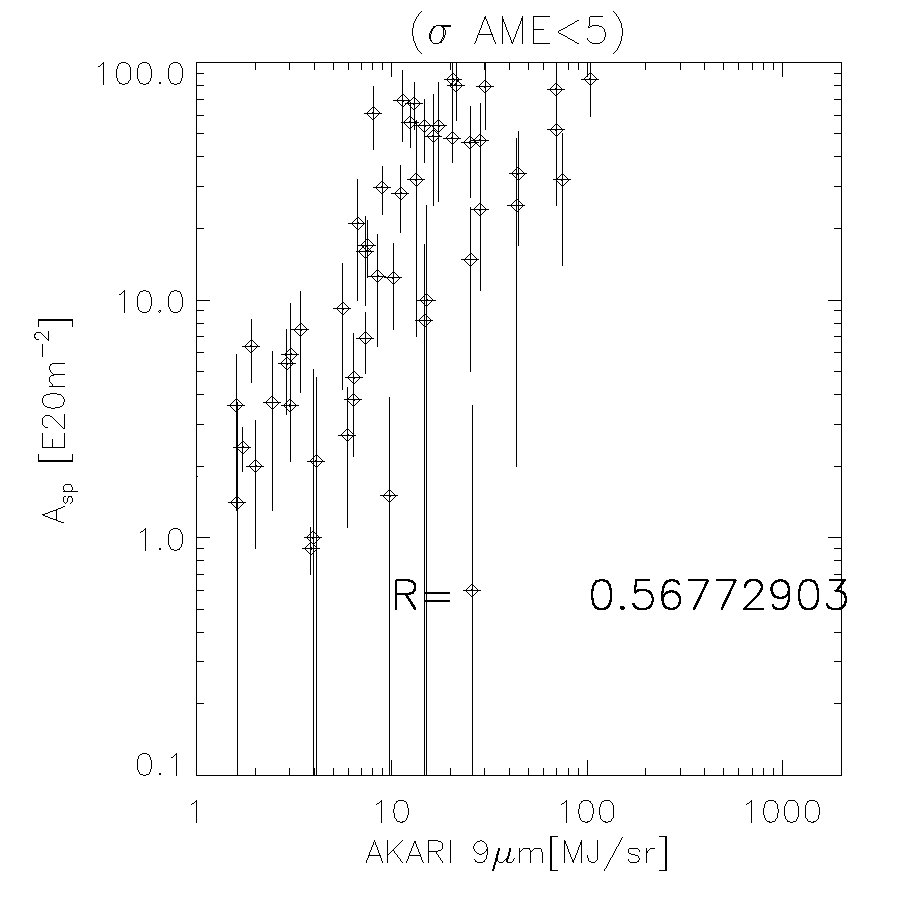
\includegraphics[width=50mm]{IRIntMWAmp/akari9_Asp_nosp.pdf}
  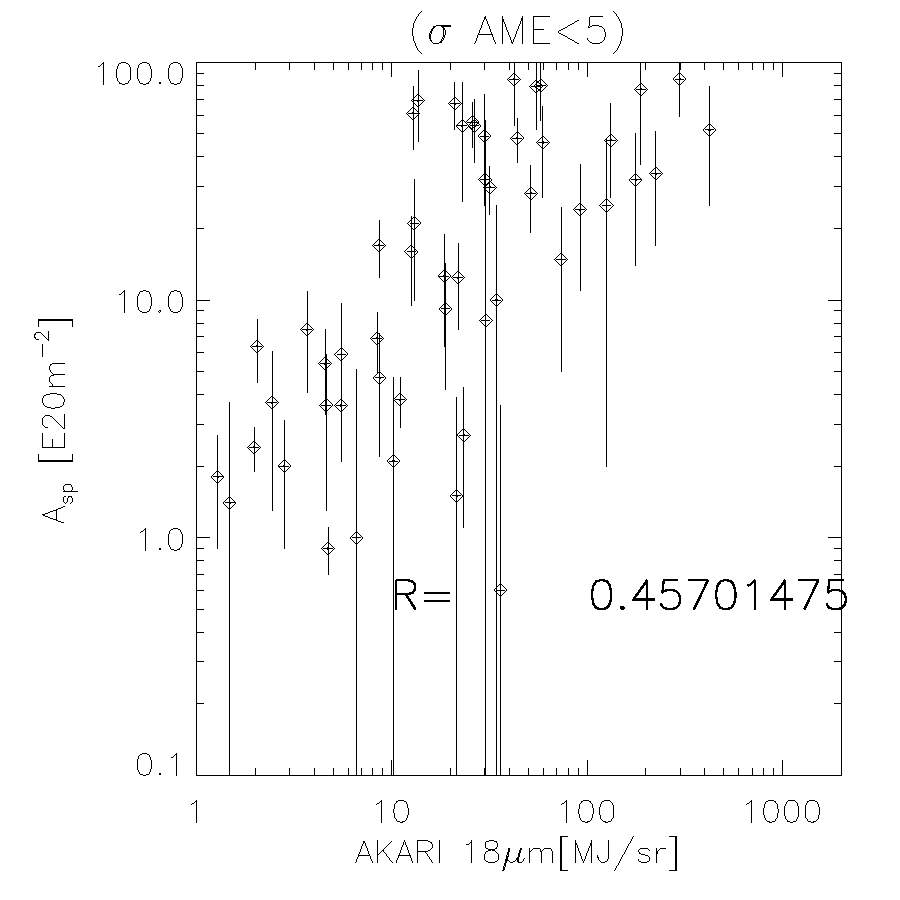
\includegraphics[width=50mm]{IRIntMWAmp/akari18_Asp_nosp.pdf}
  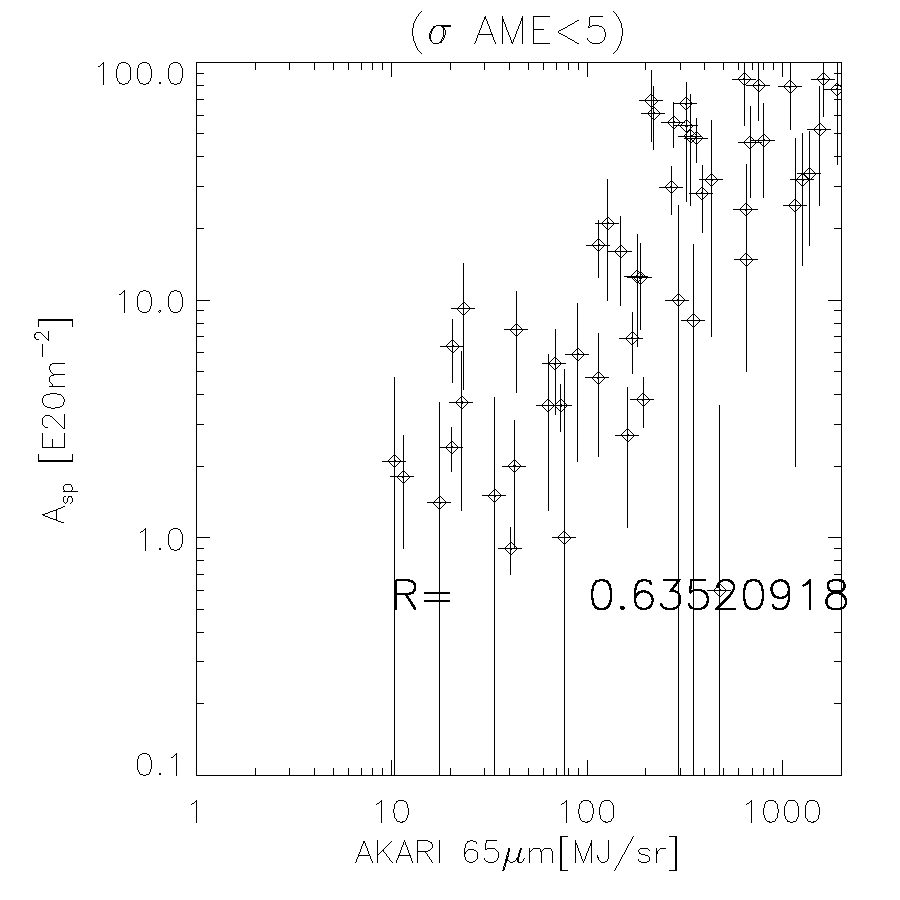
\includegraphics[width=50mm]{IRIntMWAmp/akari65_Asp_nosp.pdf}
  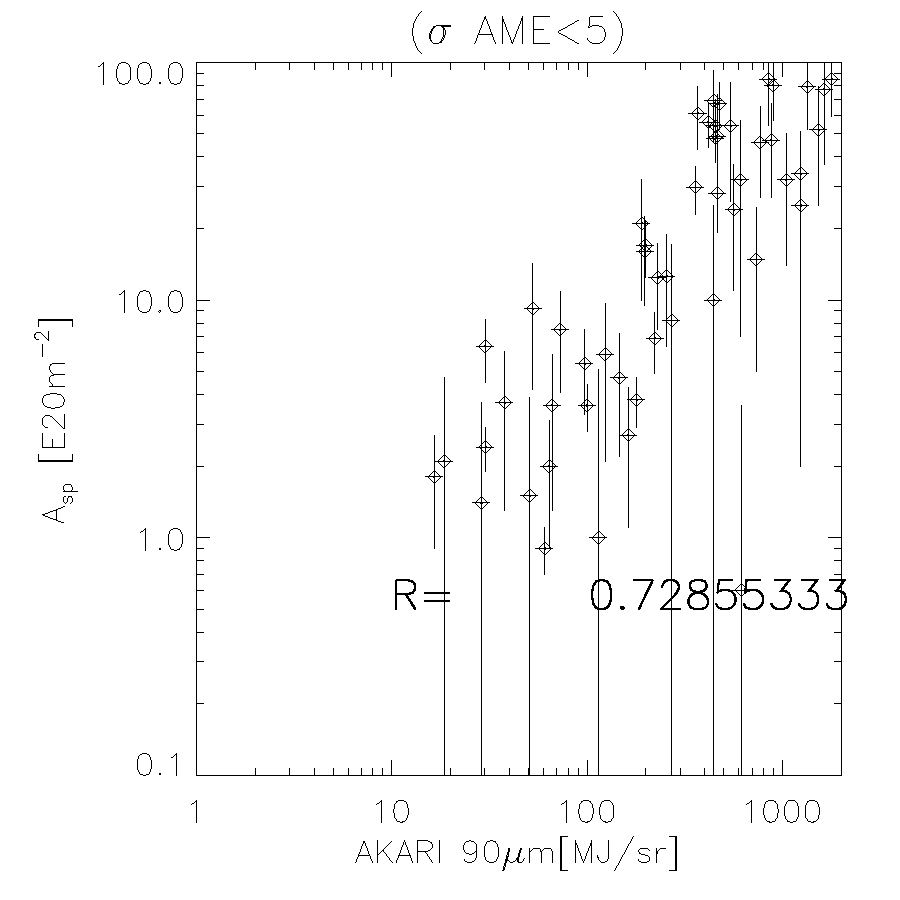
\includegraphics[width=50mm]{IRIntMWAmp/akari90_Asp_nosp.pdf}
  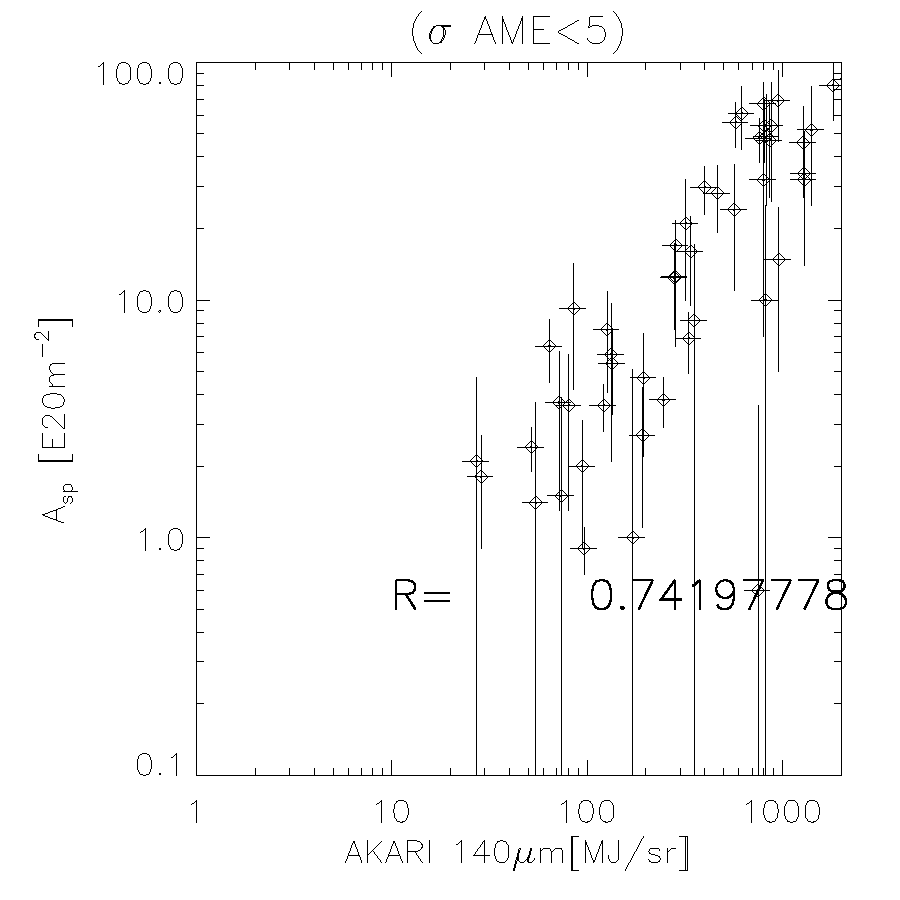
\includegraphics[width=50mm]{IRIntMWAmp/akari140_Asp_nosp.pdf}
  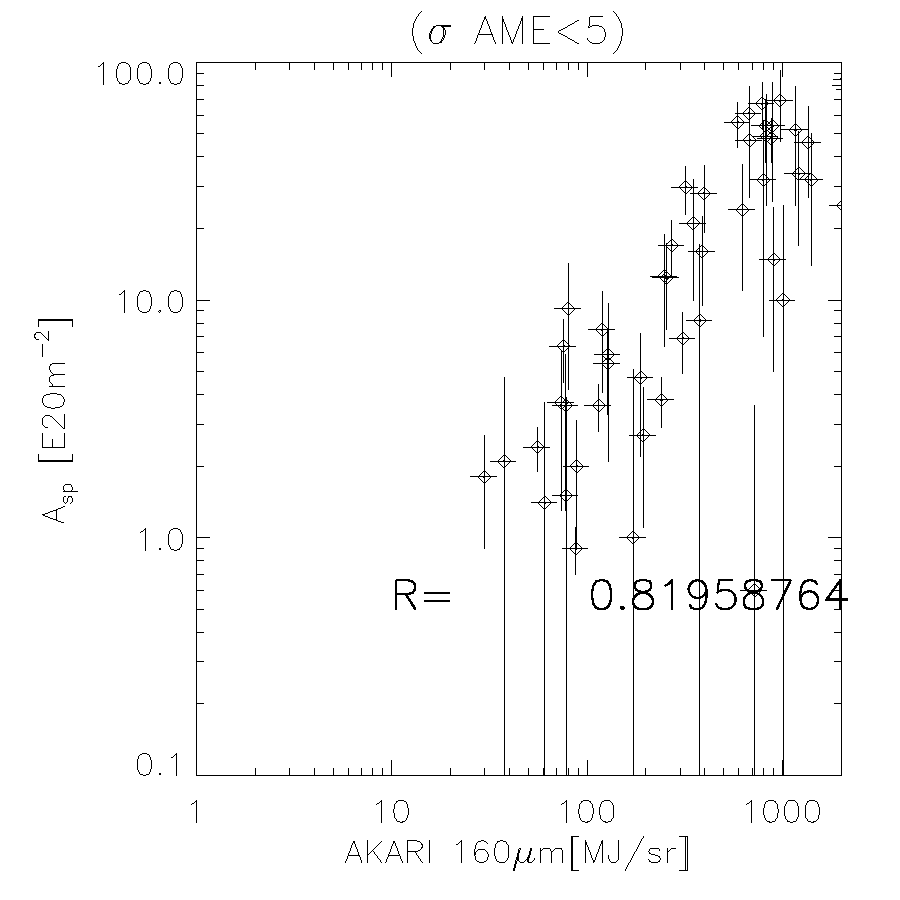
\includegraphics[width=50mm]{IRIntMWAmp/akari160_Asp_nosp.pdf}
  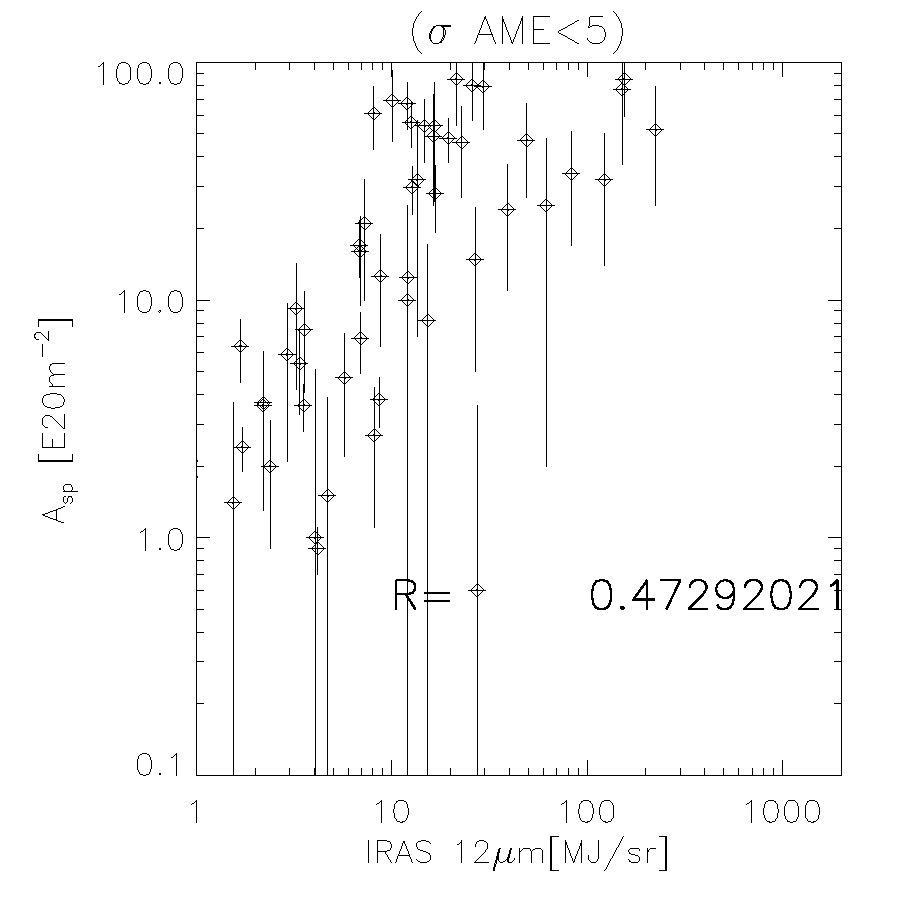
\includegraphics[width=50mm]{IRIntMWAmp/iras12_Asp_nosp.pdf}
  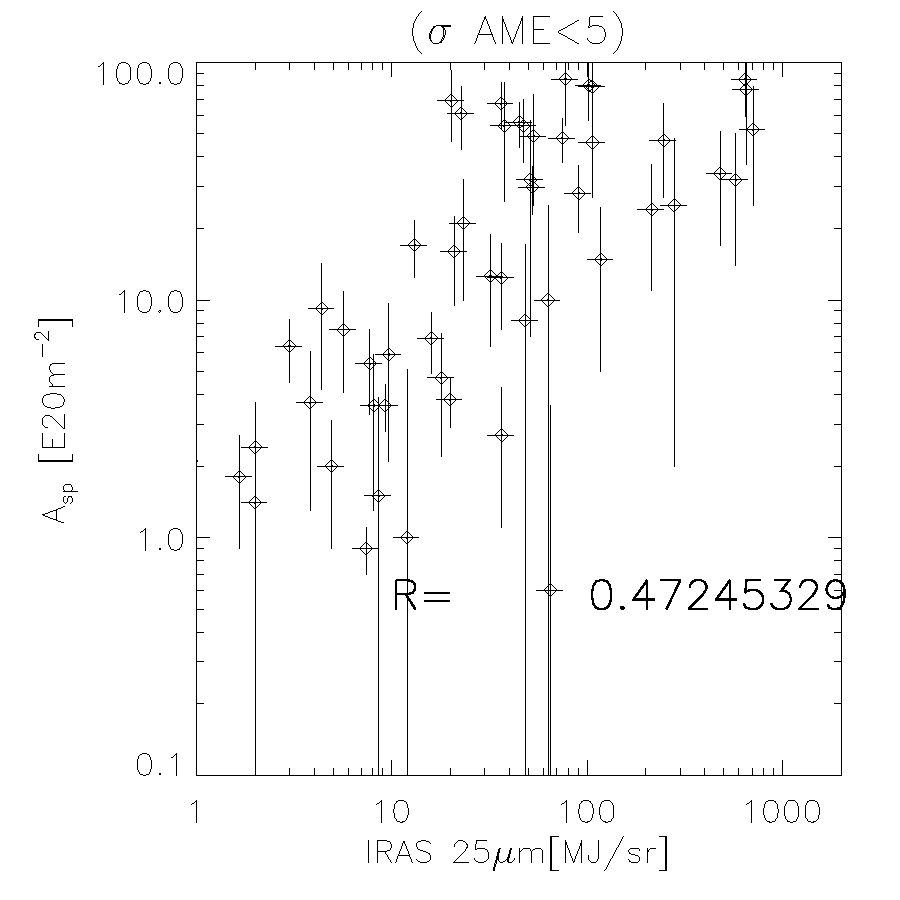
\includegraphics[width=50mm]{IRIntMWAmp/iras25_Asp_nosp.pdf}
  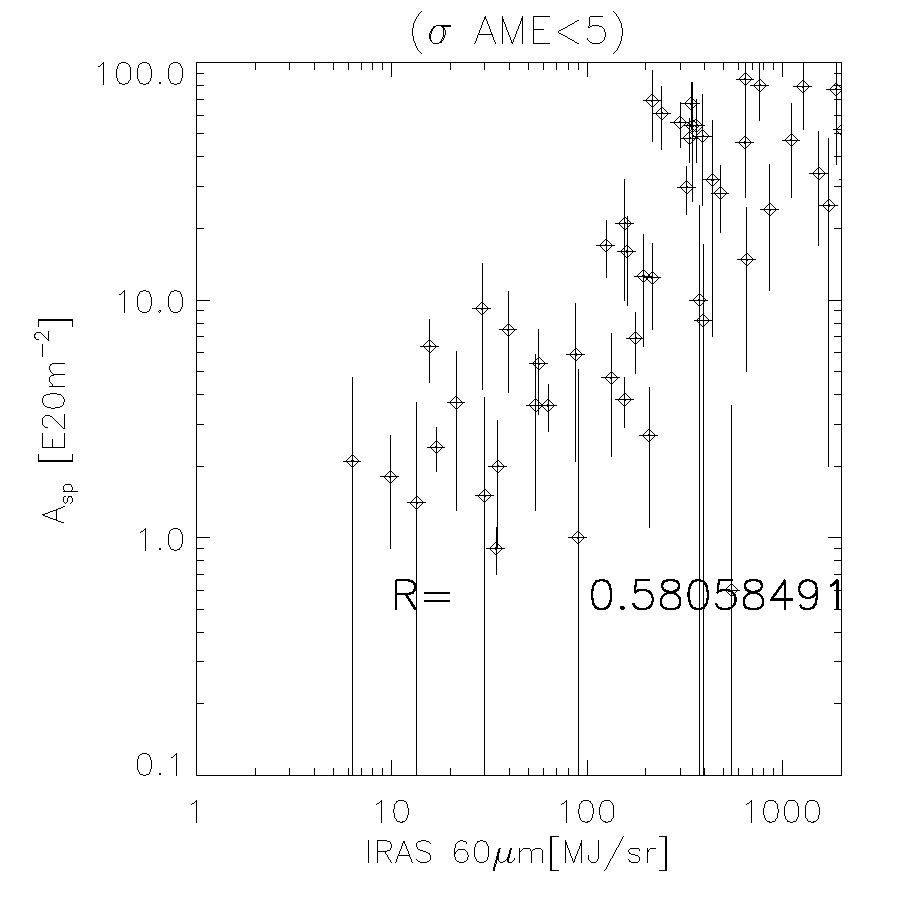
\includegraphics[width=50mm]{IRIntMWAmp/iras60_Asp_nosp.pdf}
  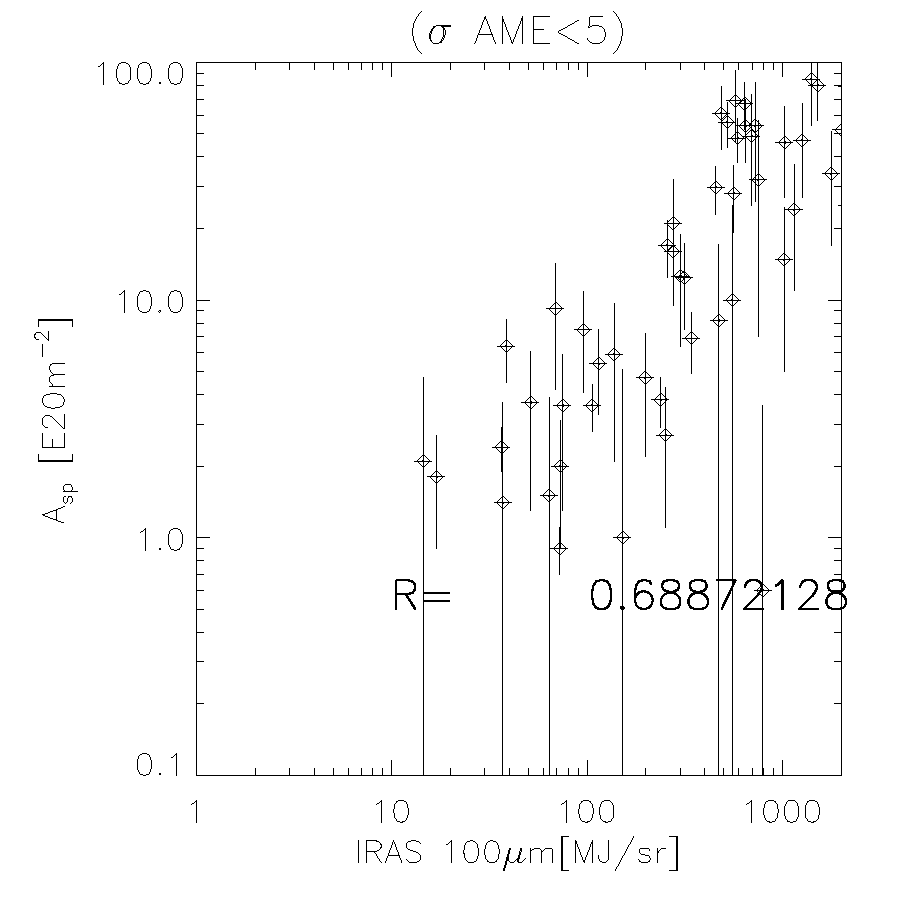
\includegraphics[width=50mm]{IRIntMWAmp/iras100_Asp_nosp.pdf}
  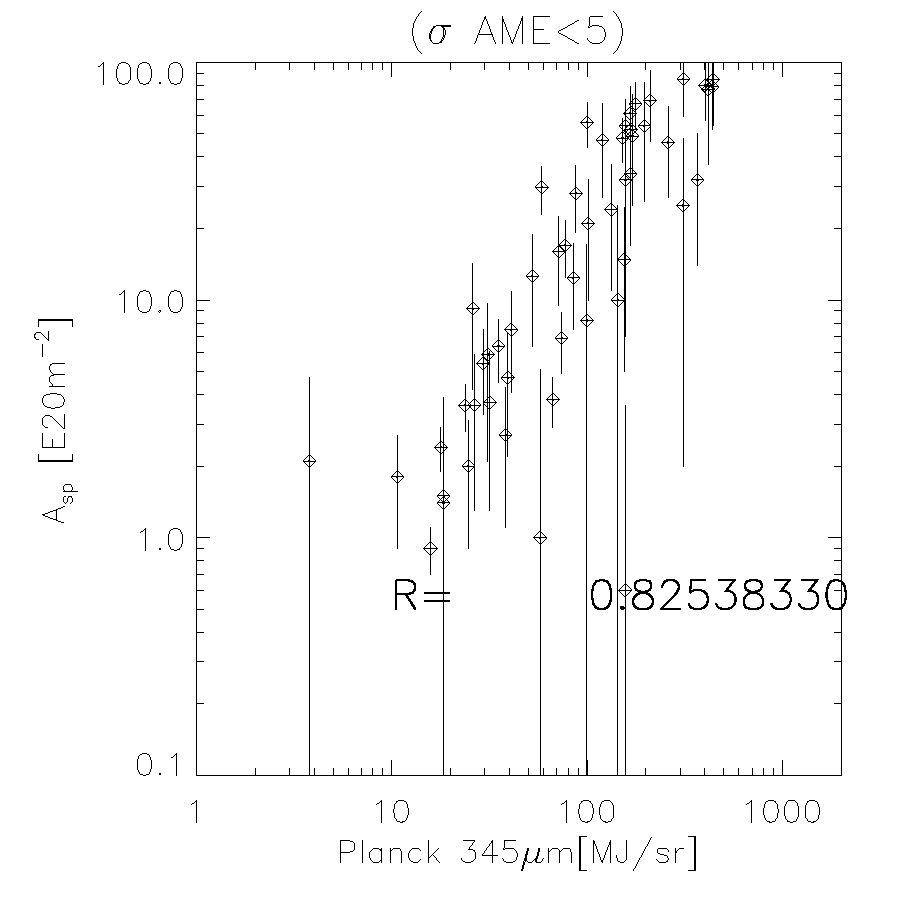
\includegraphics[width=50mm]{IRIntMWAmp/planck857_Asp_nosp.pdf}
  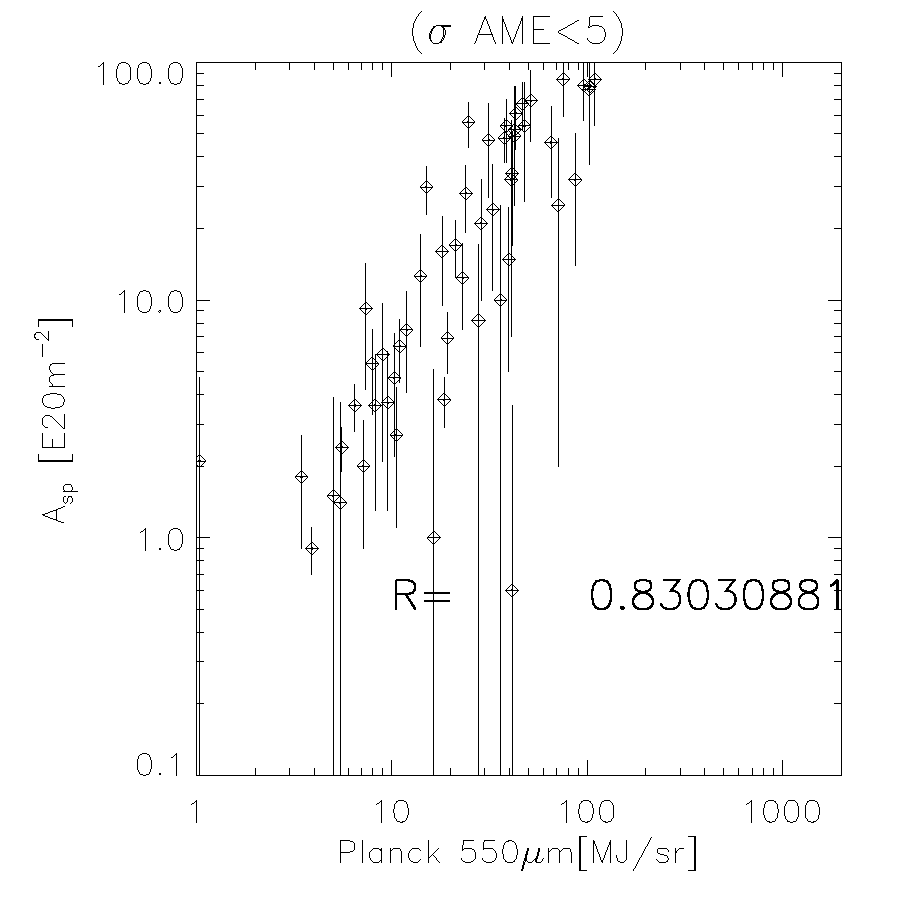
\includegraphics[width=50mm]{IRIntMWAmp/planck545_Asp_nosp.pdf}
\caption{These plots show the $I({\lambda})$ vs, $A_{sp}$ when only the non-significant AME regions are considered ($\sigma AME < 5$). 
}
\label{fig:IRIntMWAmpnosp}
\end{figure}

\subsection{Average Infrared Intensity $I({\lambda})$ Scaled by $G0$ vs. AME Amplitude $A_{sp}$}
     Following the analysis of previous studies, we plotted these regions again though with the intensities scaled by the $G0$ value of each region. $G0$ is the ISRF of a region relative to that of the solar neighborhood, and is determined from the modified blackbody fitting described in Chapter 2. 
\begin{figure}[!htb]
\centering
 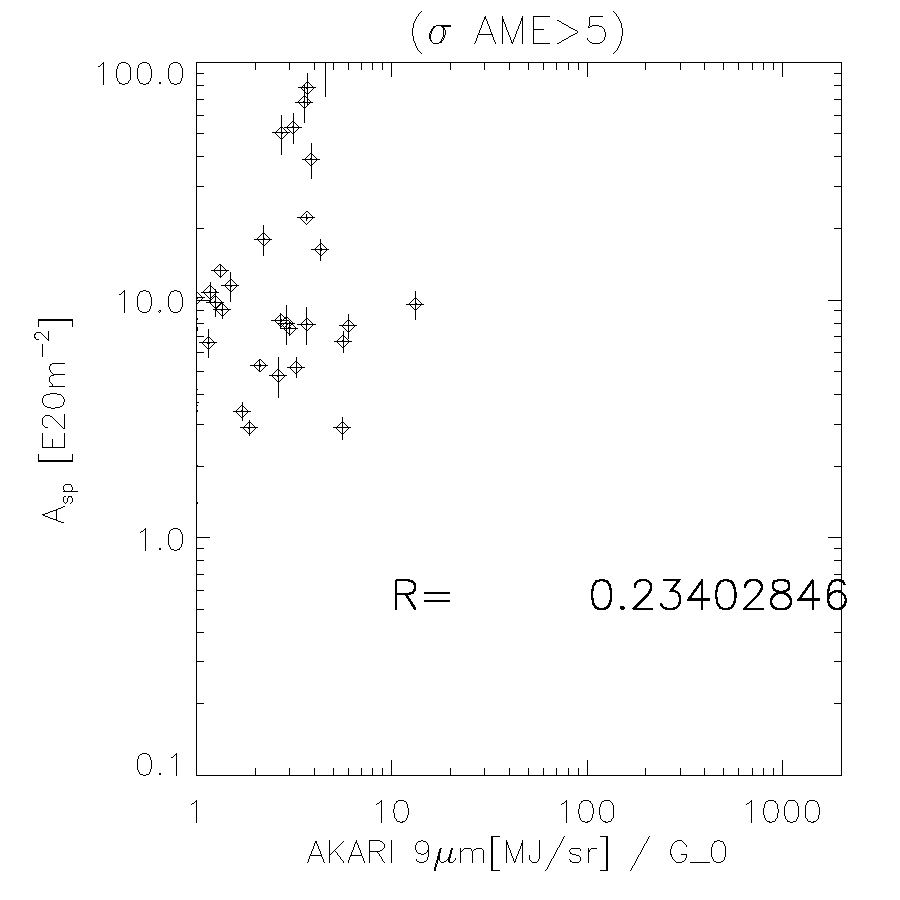
\includegraphics[width=50mm]{IRIntG0MWAmp/akari9G0_Asp_sp.pdf}
  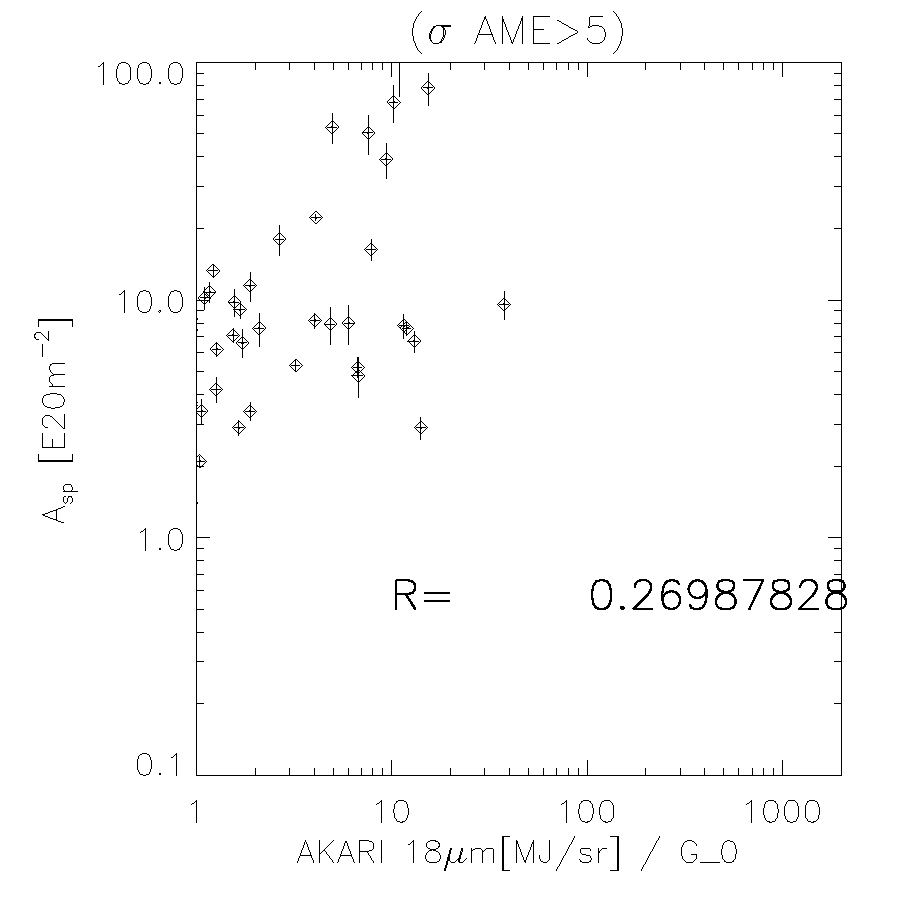
\includegraphics[width=50mm]{IRIntG0MWAmp/akari18G0_Asp_sp.pdf}
  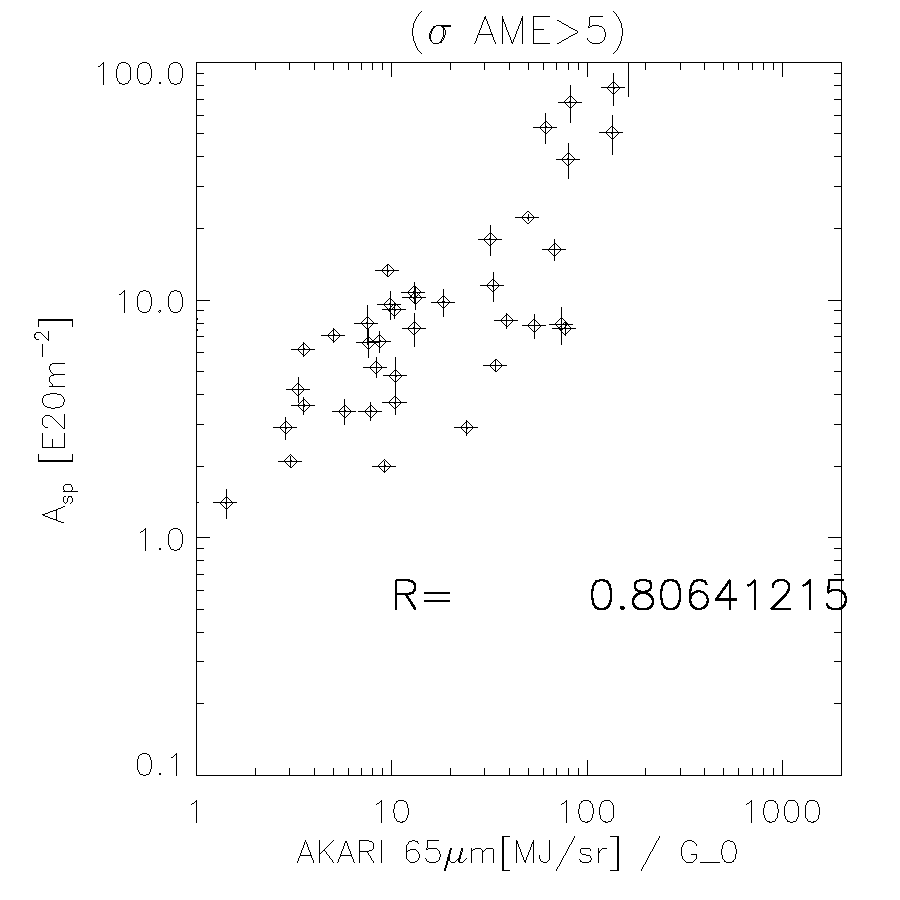
\includegraphics[width=50mm]{IRIntG0MWAmp/akari65G0_Asp_sp.pdf}
  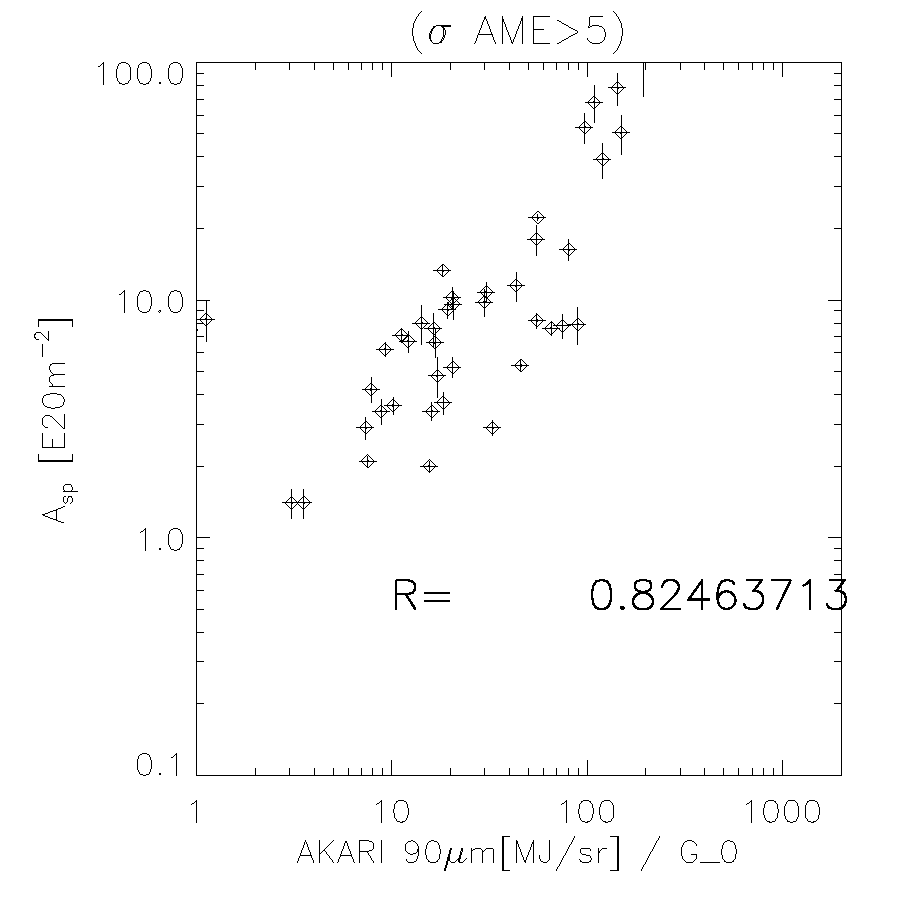
\includegraphics[width=50mm]{IRIntG0MWAmp/akari90G0_Asp_sp.pdf}
  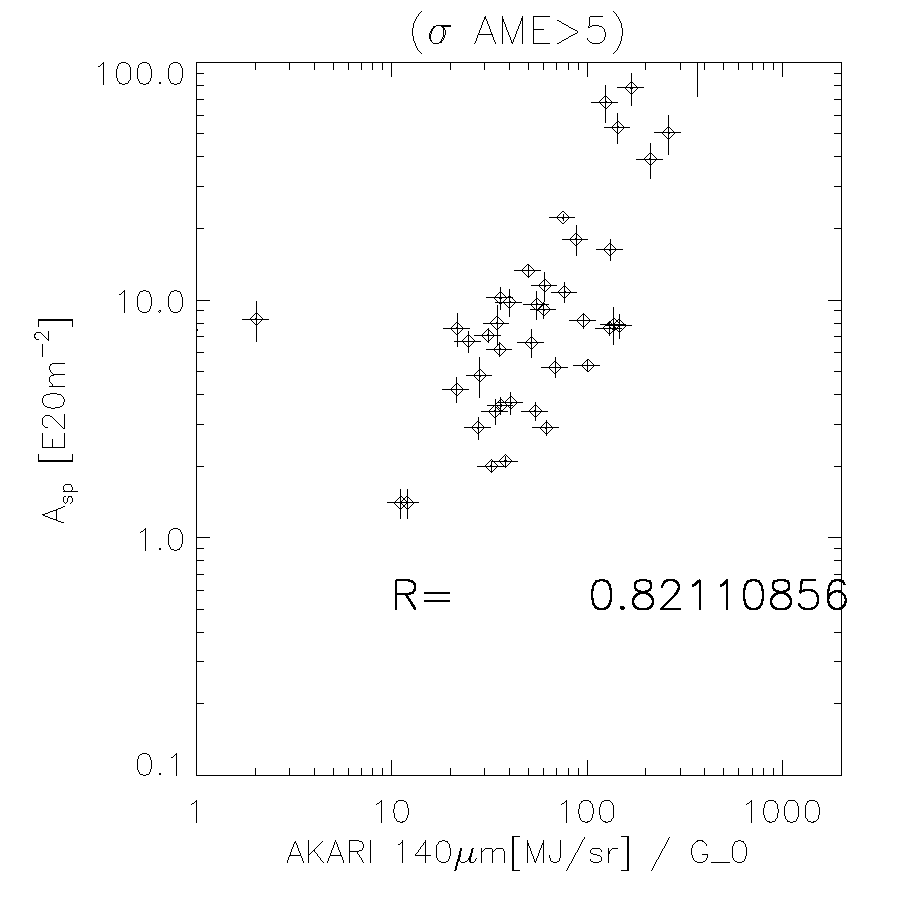
\includegraphics[width=50mm]{IRIntG0MWAmp/akari140G0_Asp_sp.pdf}
  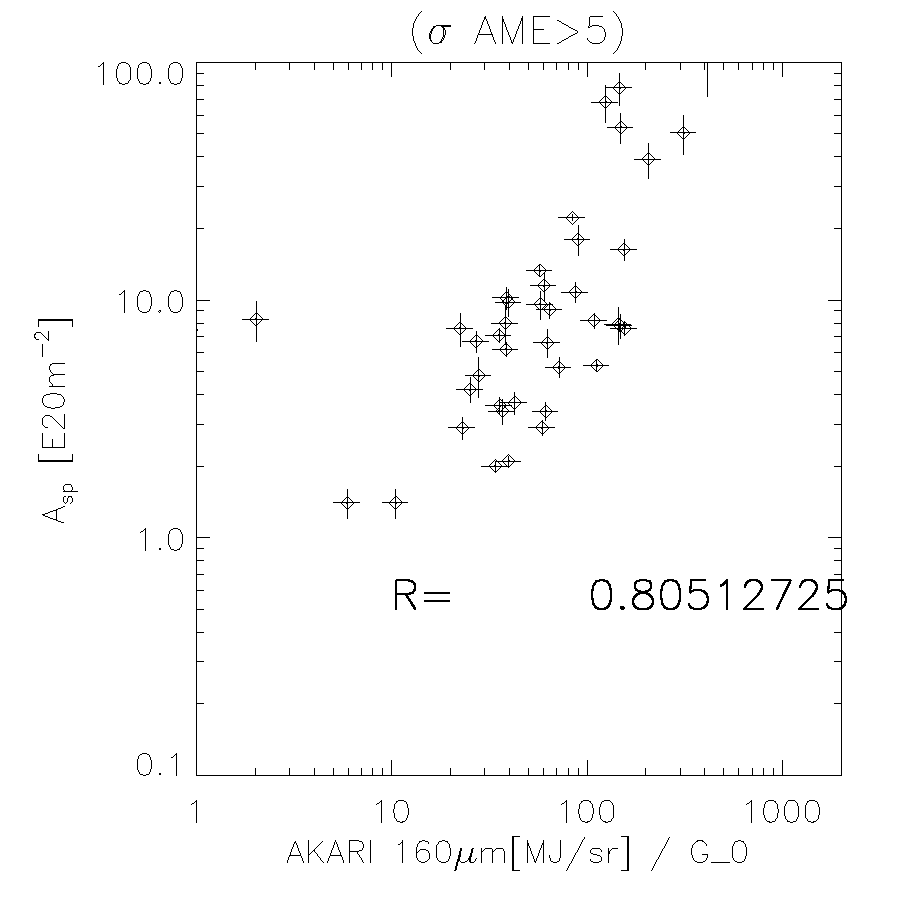
\includegraphics[width=50mm]{IRIntG0MWAmp/akari160G0_Asp_sp.pdf}
  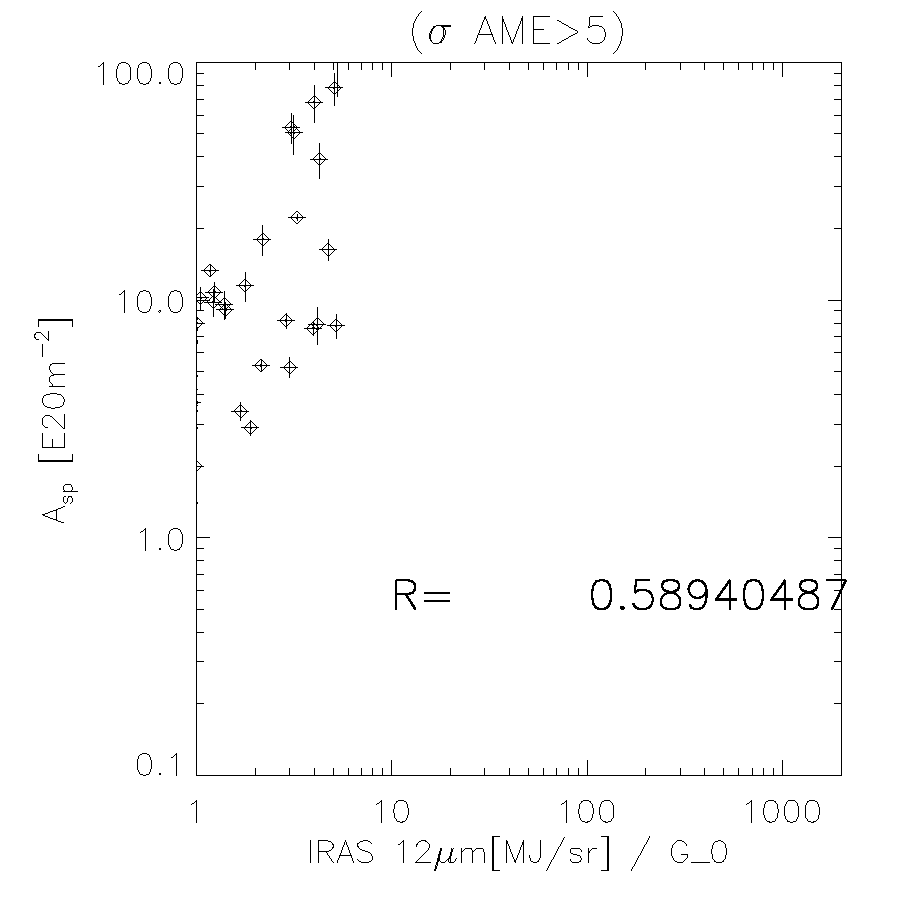
\includegraphics[width=50mm]{IRIntG0MWAmp/iras12G0_Asp_sp.pdf}
  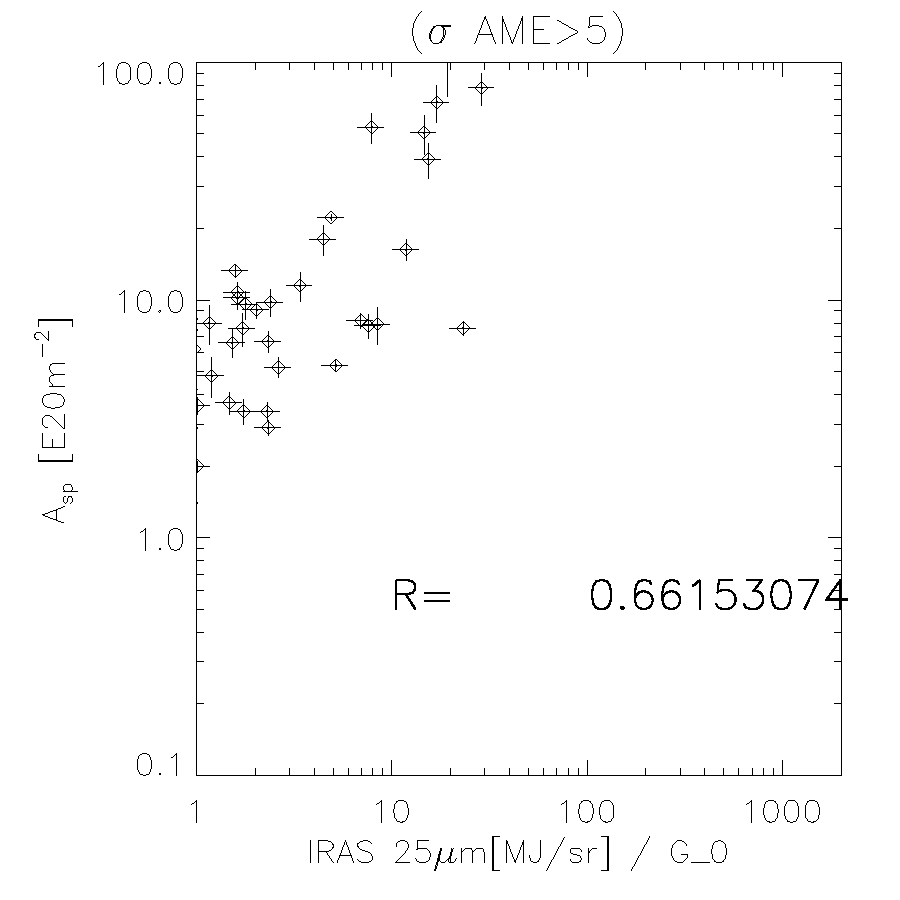
\includegraphics[width=50mm]{IRIntG0MWAmp/iras25G0_Asp_sp.pdf}
  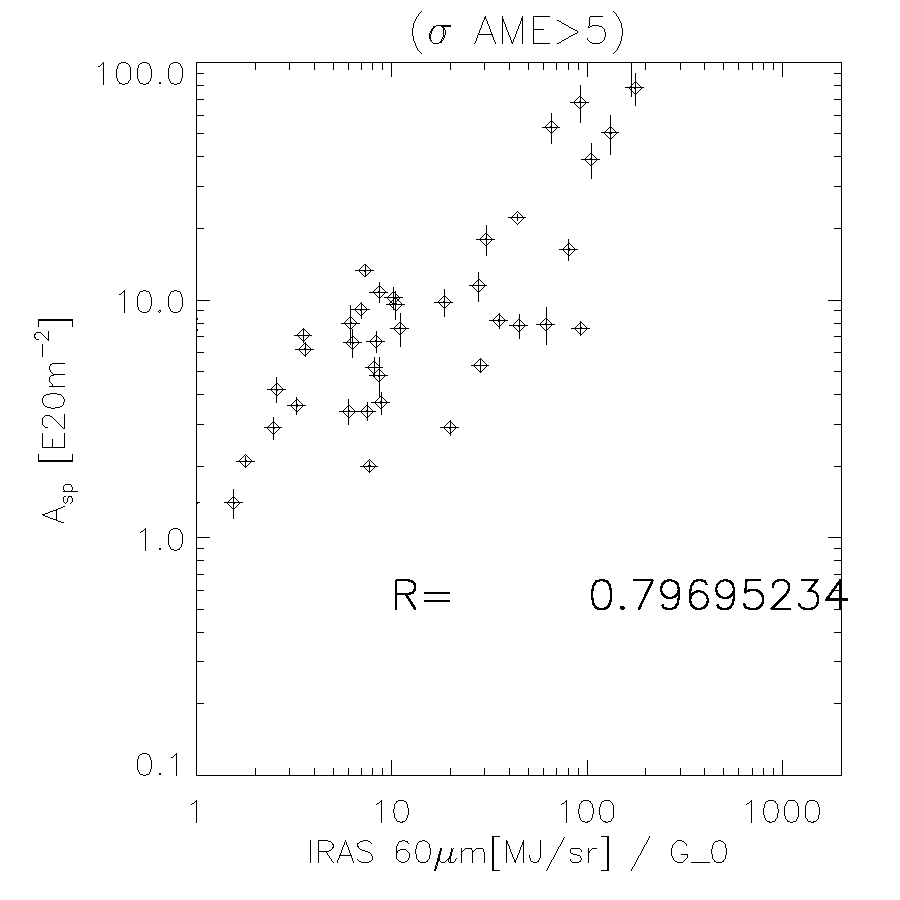
\includegraphics[width=50mm]{IRIntG0MWAmp/iras60G0_Asp_sp.pdf}
  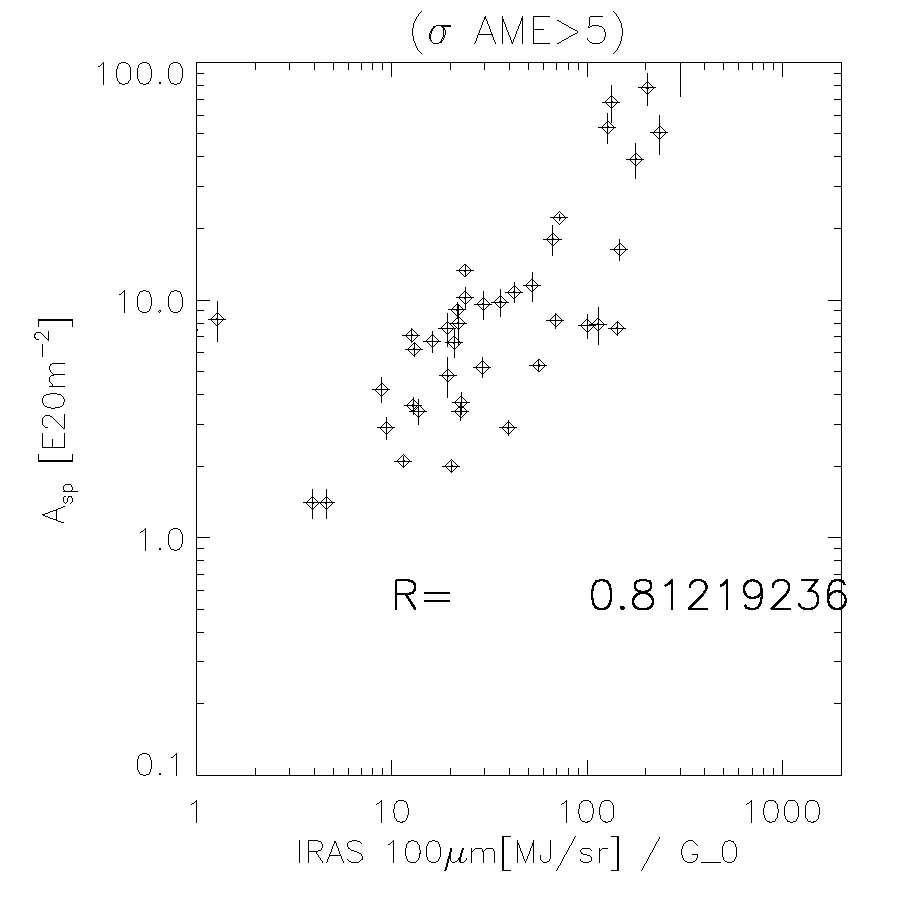
\includegraphics[width=50mm]{IRIntG0MWAmp/iras100G0_Asp_sp.pdf}
  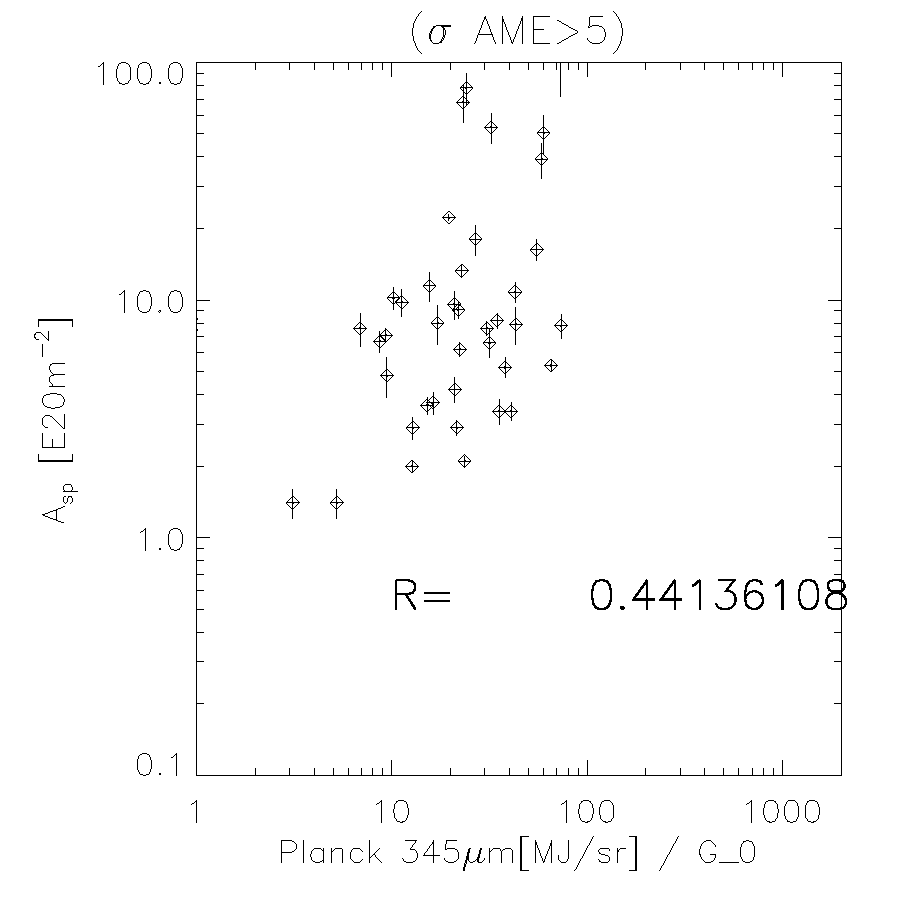
\includegraphics[width=50mm]{IRIntG0MWAmp/planck857G0_Asp_sp.pdf}
  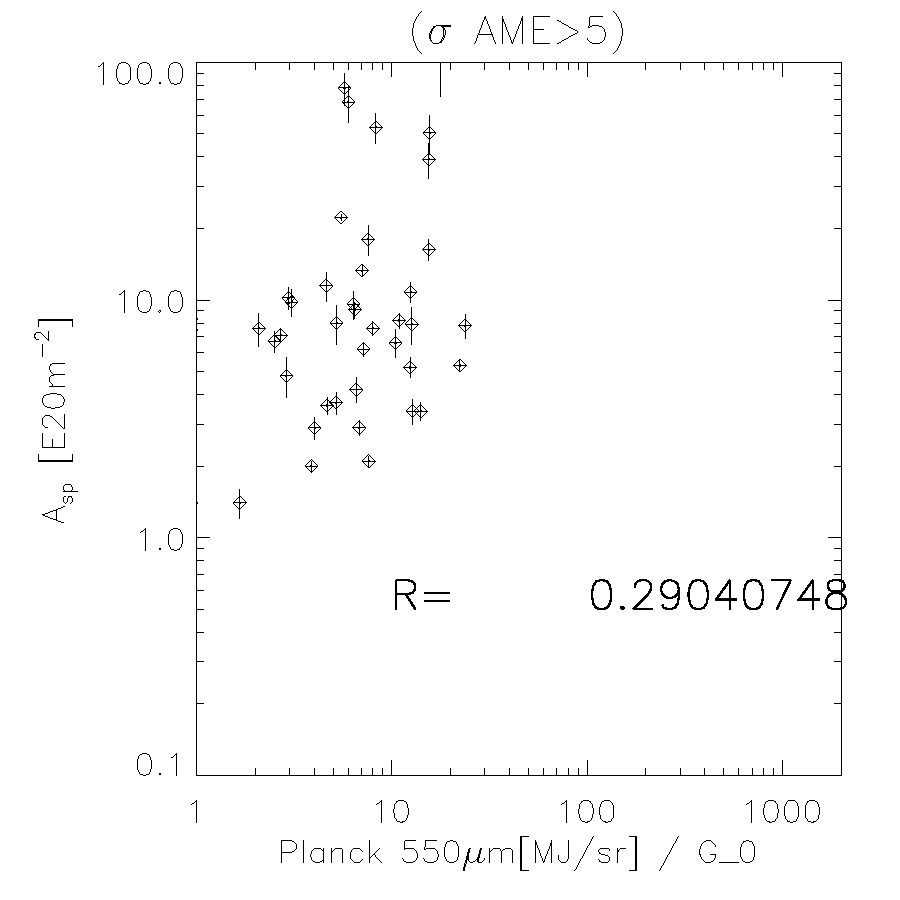
\includegraphics[width=50mm]{IRIntG0MWAmp/planck545G0_Asp_sp.pdf}
\caption{In these figures, the band-by-band correlation test of $I({\lambda})$ vs. $A_{sp}$ is repeated, dividing $I({\lambda})$ by $G0$. Only significant AME regions are considered here ($\sigma AME < 5$). This case shows the weakest correlation of AKARI 9~$\mu$m with $A_{sp}$.
}
\label{fig:IRIntG0MWAmpsp}
\end{figure}
\begin{figure}[!htb]
\centering
 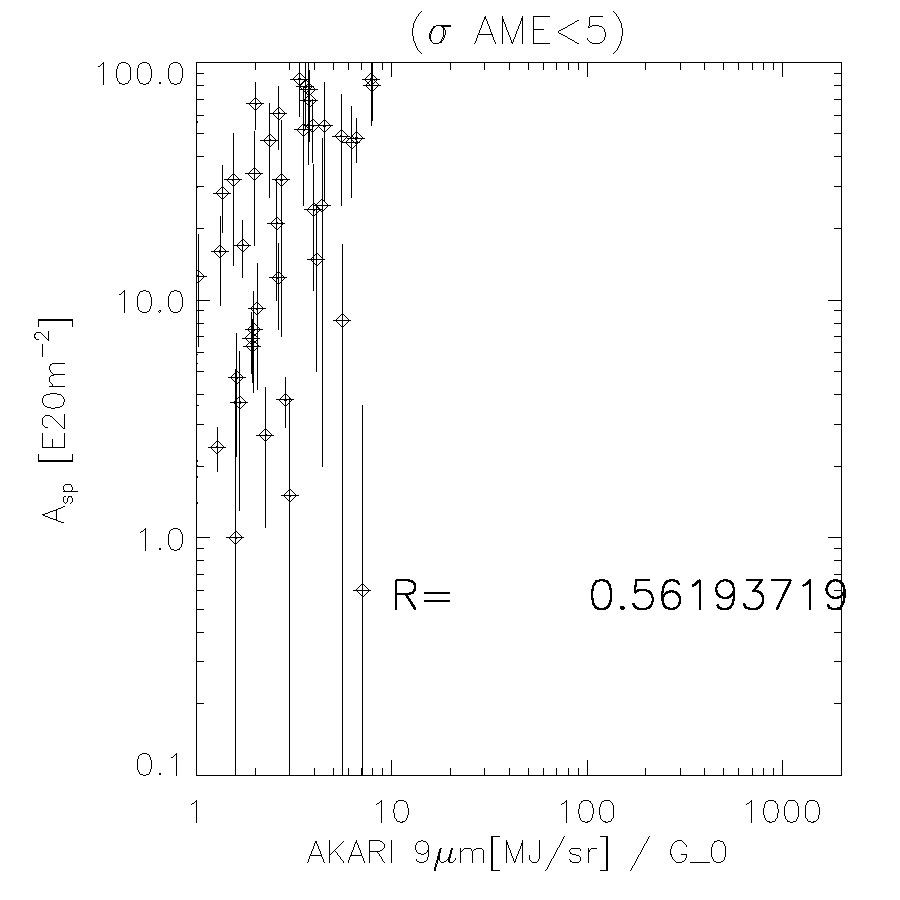
\includegraphics[width=50mm]{IRIntG0MWAmp/akari9G0_Asp_nosp.pdf}
  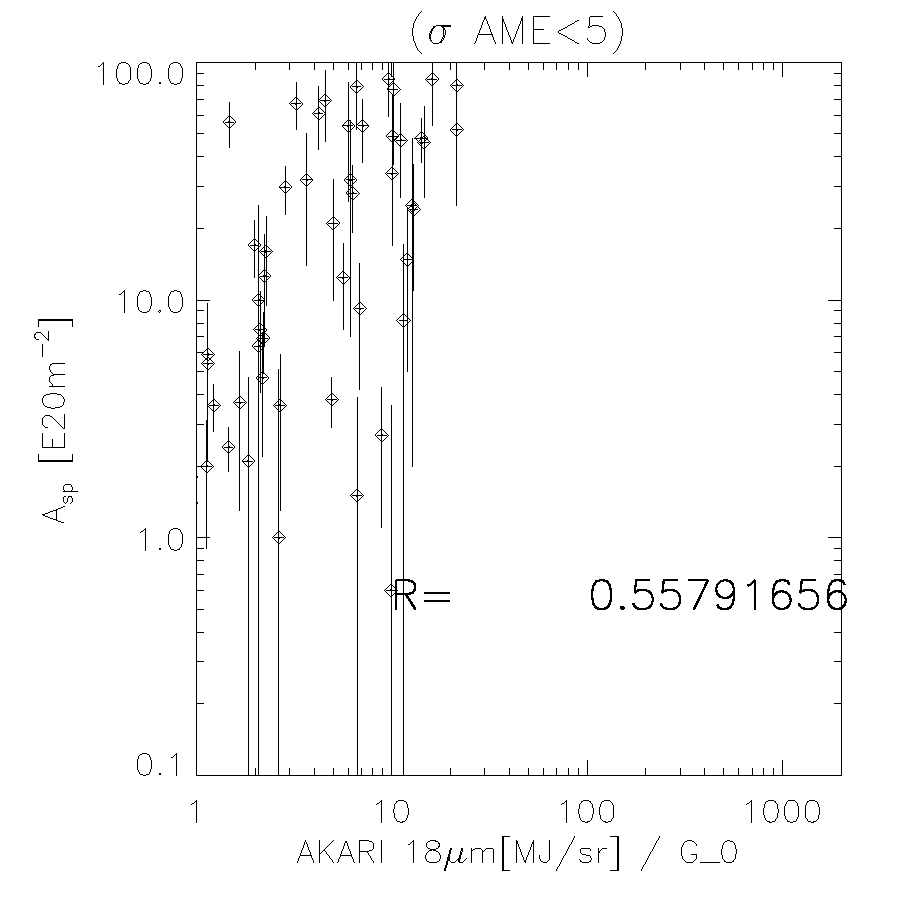
\includegraphics[width=50mm]{IRIntG0MWAmp/akari18G0_Asp_nosp.pdf}
  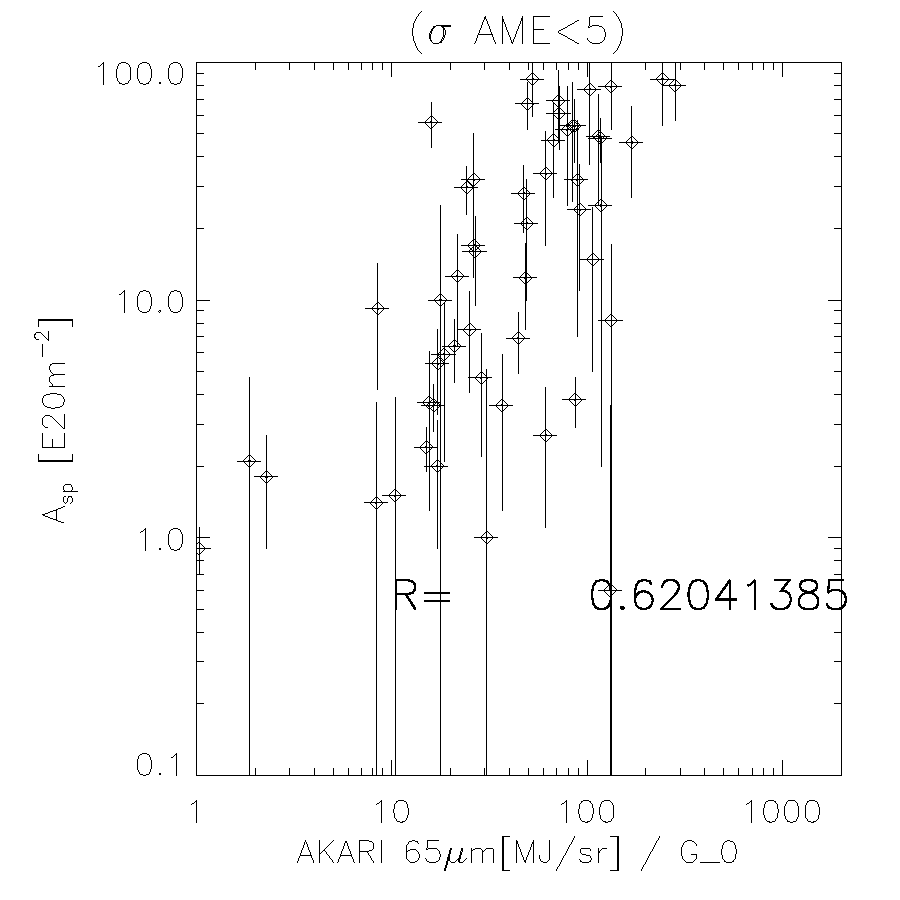
\includegraphics[width=50mm]{IRIntG0MWAmp/akari65G0_Asp_nosp.pdf}
  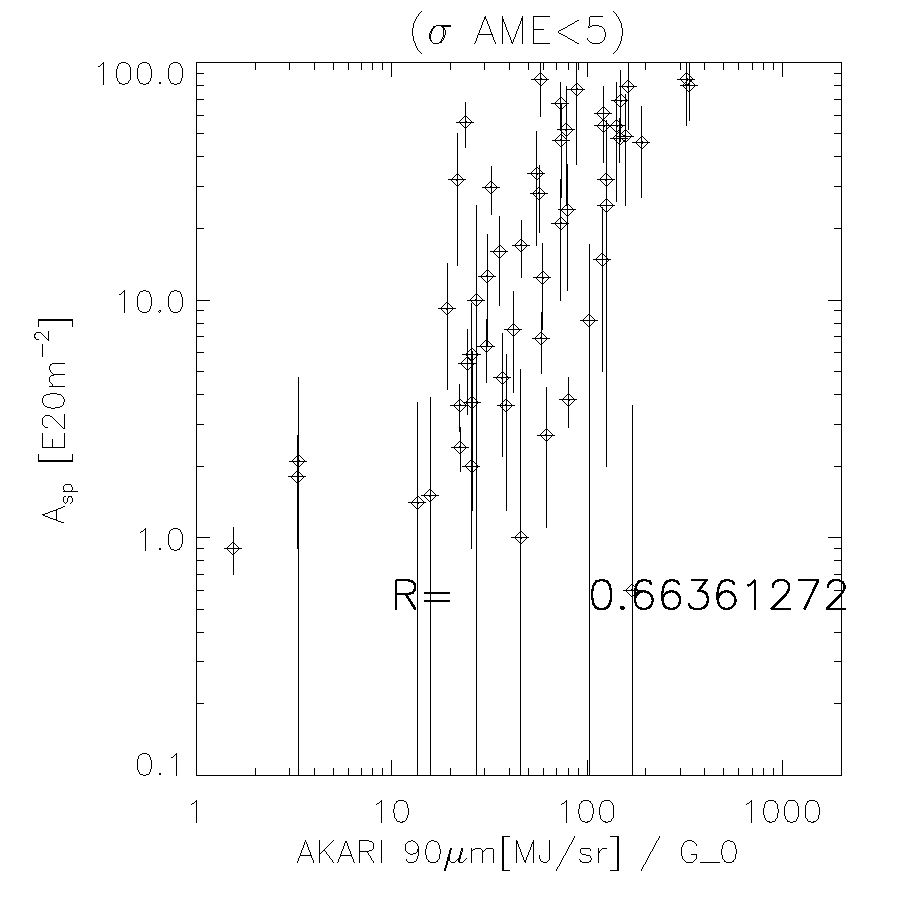
\includegraphics[width=50mm]{IRIntG0MWAmp/akari90G0_Asp_nosp.pdf}
  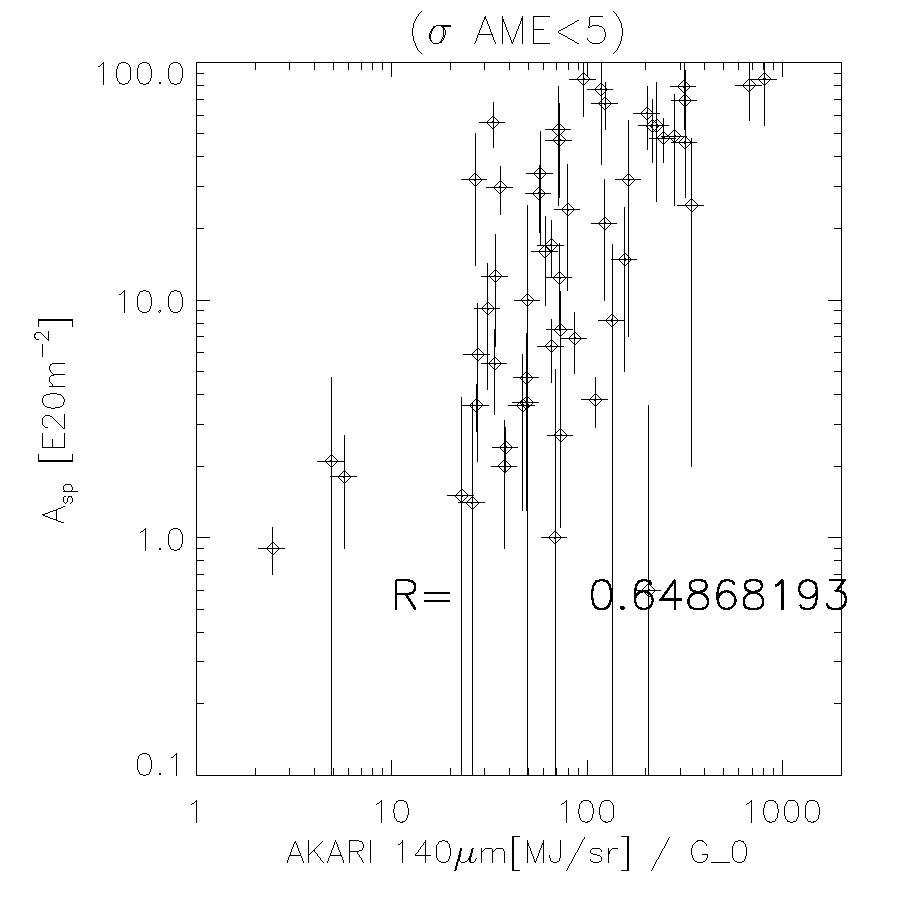
\includegraphics[width=50mm]{IRIntG0MWAmp/akari140G0_Asp_nosp.pdf}
  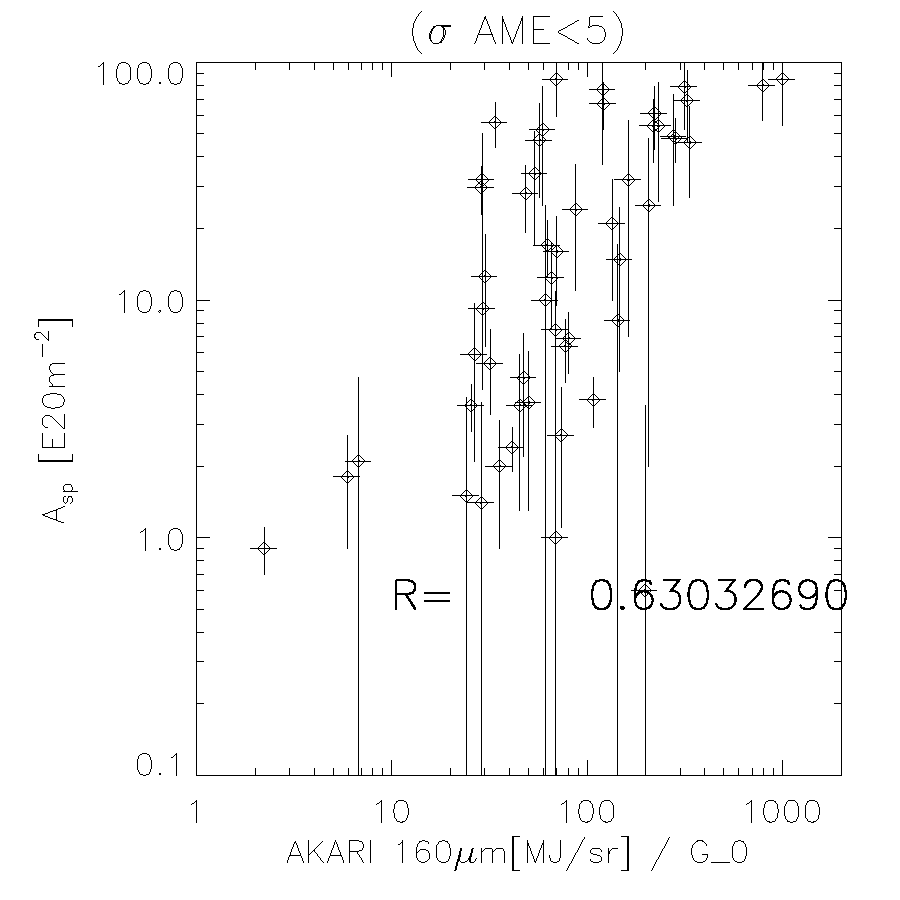
\includegraphics[width=50mm]{IRIntG0MWAmp/akari160G0_Asp_nosp.pdf}
  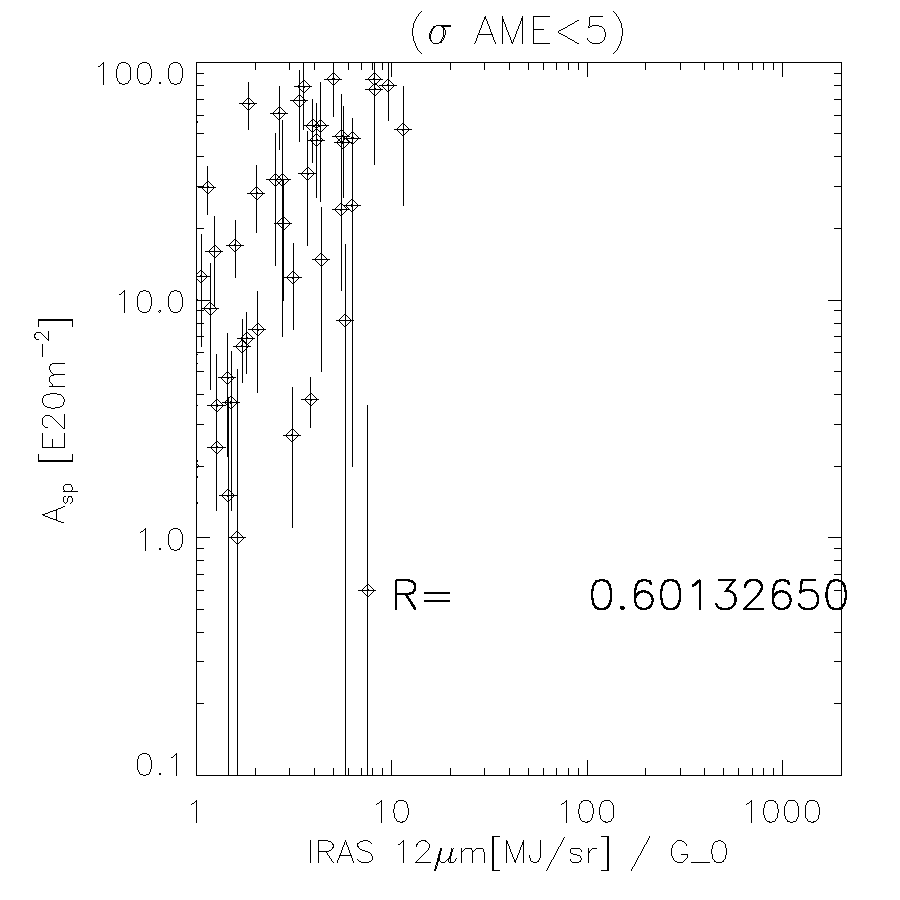
\includegraphics[width=50mm]{IRIntG0MWAmp/iras12G0_Asp_nosp.pdf}
  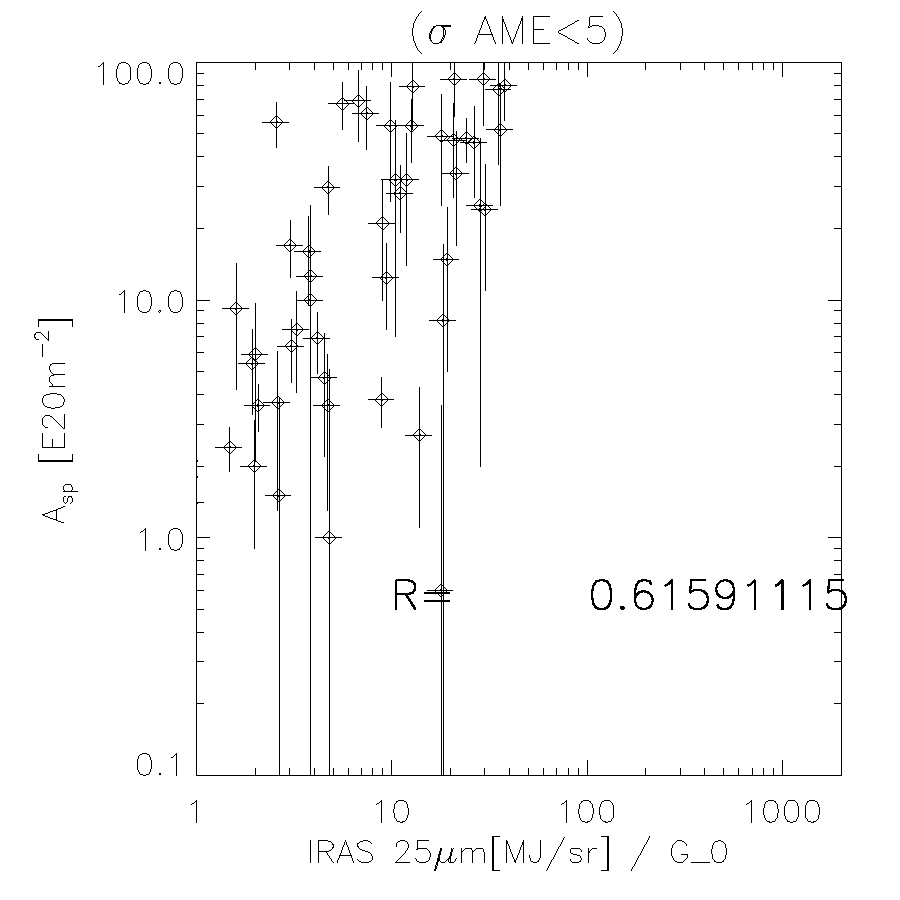
\includegraphics[width=50mm]{IRIntG0MWAmp/iras25G0_Asp_nosp.pdf}
  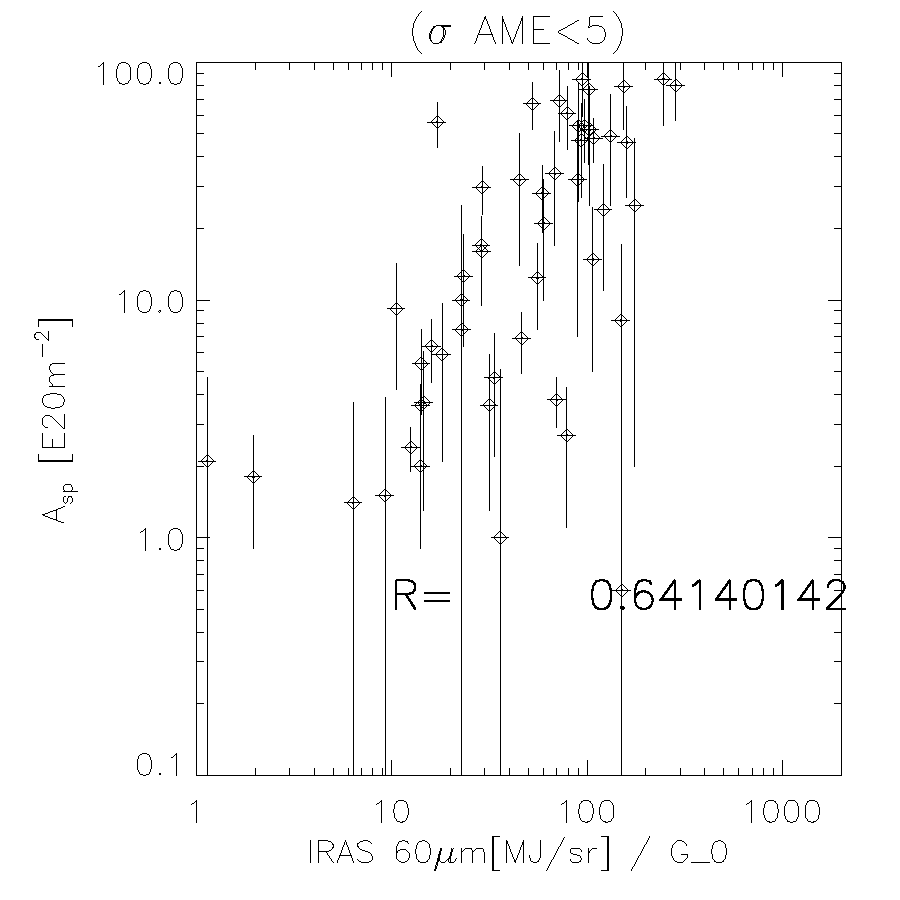
\includegraphics[width=50mm]{IRIntG0MWAmp/iras60G0_Asp_nosp.pdf}
  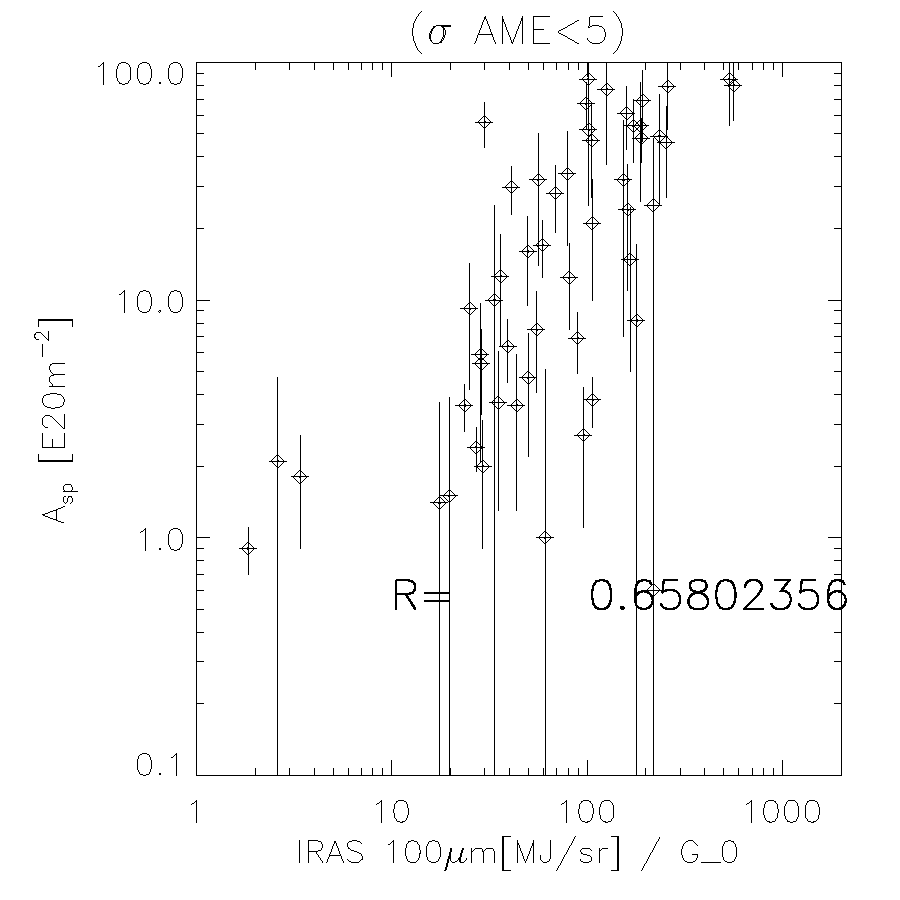
\includegraphics[width=50mm]{IRIntG0MWAmp/iras100G0_Asp_nosp.pdf}
  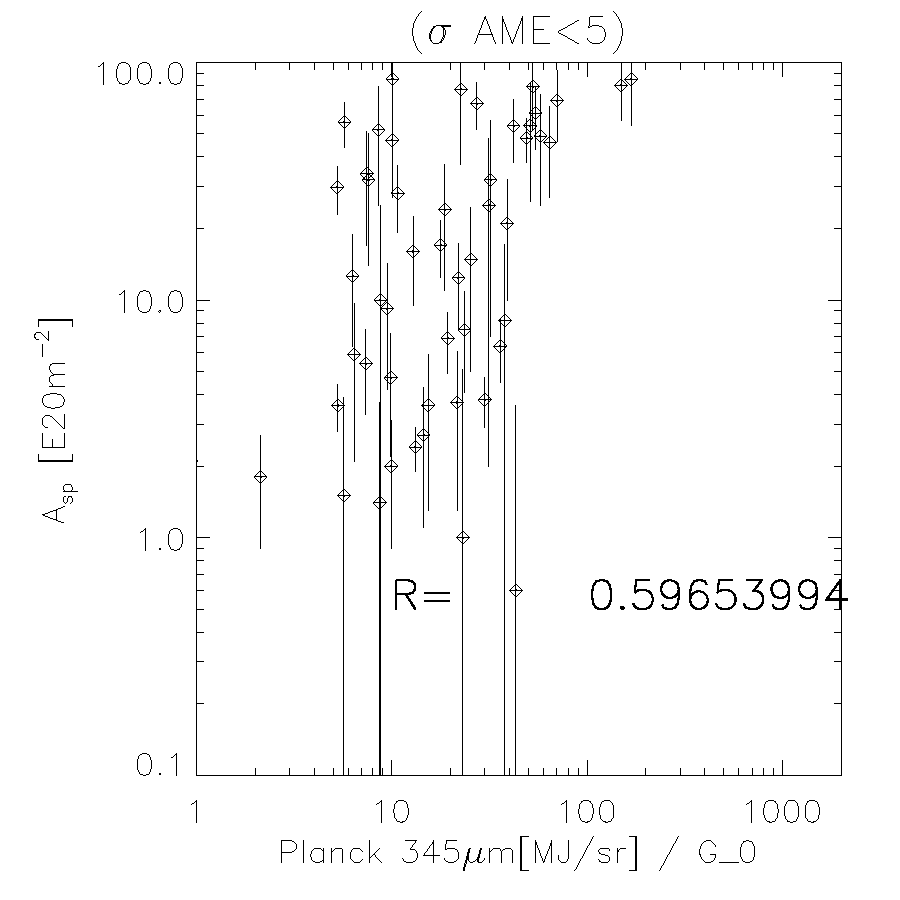
\includegraphics[width=50mm]{IRIntG0MWAmp/planck857G0_Asp_nosp.pdf}
  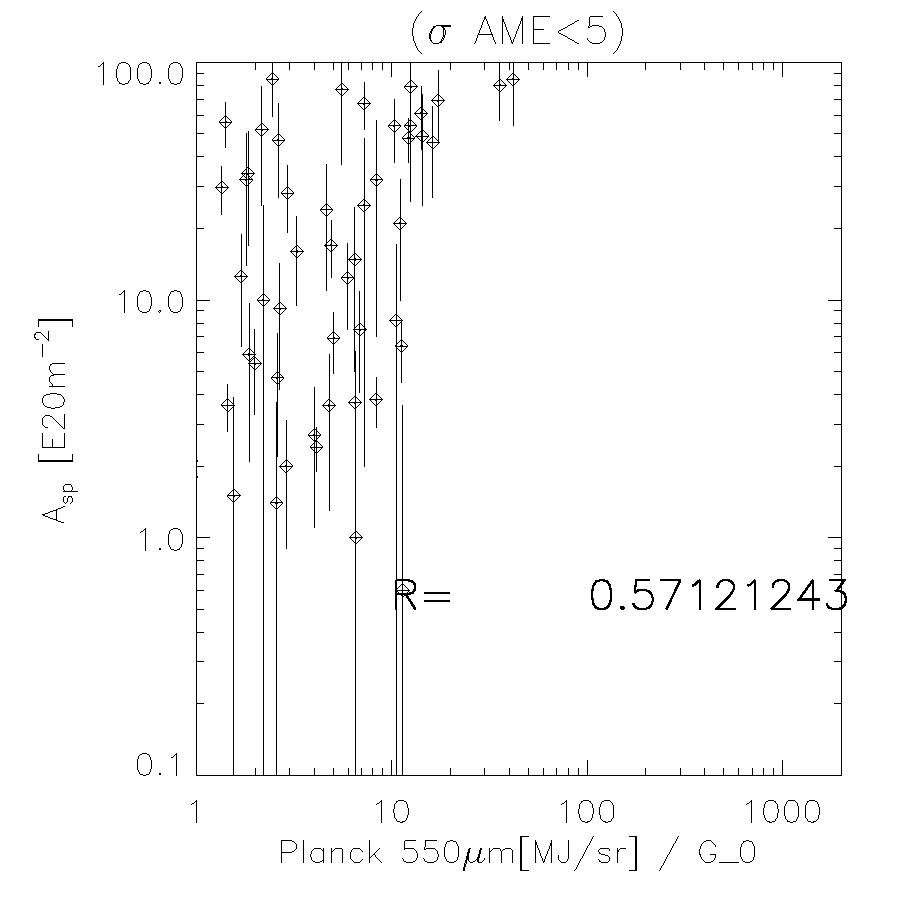
\includegraphics[width=50mm]{IRIntG0MWAmp/planck545G0_Asp_nosp.pdf}
\caption{In these figures, the band-by-band correlation test of $I({\lambda})$ vs. $A_{sp}$ is repeated, dividing $I({\lambda})$ by $G0$. Only non-significant AME regions are plotted here. This case shows a similar correlation factor across all of the bands. Interestingly,  the AKARI 9~$\mu$m with $A_{sp}$ correlation is stronger here than for the $\sigma AME > 5$ case.
}
\label{fig:IRIntG0MWAmpnosp}
\end{figure}
     As noted in Chapter 1, previous studies found that the AME generally correlates at dust-related IR wavelengths. We see the same overall pattern in the present study. However, contrary to previous works, we find that the correlation is not improved at the small-grain-related MIR wavelengths.
     Both PCXV and \cite{ysard10b} found that the correlations improved after dividing the IR photometric data by $G0$. We have repeated that calculation here using the average $G0$ of ROI, obtained from our a modified blackbody fitting results (with $\beta$ = 2). We find generally that all of the correlations with $A_{sp}$ weaken after dividing by $G0$. 
     In order to get a finer understanding of the IR/$G0$ vs. $A_{sp}$ variations, we again followed in the method of PCXV by separately plotting regions which are well-fitted by a spinning dust model ($\sigma AME>5$) vs. regions not well fitted by a spinning dust model ($\sigma AME<5$). The results are tabulated below.
\begin{table}[!htb]
\caption{Correlation Coefficients ($R$) of $I({\lambda})$ vs. $A_{sp}$ for 98 AME Regions} \label{IRvsAspTab}
\centering
\begin{tabular}{lrrrr}
\toprule
Wavelength ($\mu$m)	&$A_{sp}$ vs. $I({\lambda})$)	&$A_{sp}$ vs. $I({\lambda})$	&$A_{sp}$ vs. $I({\lambda}$/$G0$)	&$A_{sp}$ vs. $I({\lambda})$/$G0$ \\ 
    &$\sigma AME>5$  &$\sigma AME<5$ &$\sigma AME>5$  &$\sigma AME<5$      \\
\midrule
9	&0.703	&0.568	&0.234	&0.562 \\
12	&0.735	&0.473	&0.270	&0.601 \\
18	&0.649	&0.457	&0.589	&0.558 \\
25	&0.659	&0.472	&0.662	&0.616 \\
60	&0.761	&0.580	&0.797	&0.641 \\
65	&0.811	&0.635	&0.806	&0.701 \\
90	&0.851	&0.729	&0.824	&0.728 \\
100	&0.871	&0.689	&0.812	&0.658 \\
140	&0.944	&0.742	&0.821	&0.649 \\
160	&0.965	&0.820	&0.805	&0.630 \\
345	&0.944	&0.825	&0.441	&0.597 \\
550	&0.920	&0.830	&0.290	&0.571 \\
\bottomrule
\end{tabular}
\end{table}

\subsection{AKARI 9:18~$\mu$m Ratio vs. AME$\sigma$}
     We described a preliminary result in proceedings at the 2014 \textit{Universe in the Light of AKARI} conference at Oxford, regarding the AKARI/IRC 9 to 18~$\mu$m band ratio, R(9,18), for 10 PCXV AME regions (Table 3.2), Figure 3.7) (Bell et al., in prep). Regions of higher AME significance tended to have a R(9,18) value above unity. This relationship was revisited in the current study, for all 98 PCXV AME regions, and the updated result is shown in Figure 3.8. The previous result does not hold-up to the full sample, as we cannot find a clear trend between R(9,18) and AME significance.
\begin{table}[!htb]
\label{tab:R918a}
\caption{IRC average intensities and 9 to 18~$\mu$m band ratios of AME candidate regions}
\centering
\begin{tabular}{lrrrr}
\toprule
Target           & AME$\sigma$       & R(9,18)          &  9~$\mu$m MJysr$^{-1}$        & 18~$\mu$m MJysr$^{-1}$ \\
\midrule
G353.05+16.09   & 29.8	     & 1.37   &  0.134       & 0.098 \\
G160.26-18.62	 & 17.4	     & 1.27   &  0.0186      & 0.0147 \\
G004.24+18.09   & 15.6      & 1.10   &  0.00254     & 0.0023 \\
G107.20+05.20	 & 9.9       & 1.88   &  0.0955      & 0.0507 \\
G173.63+02.80	 & 5.6       & 1.04   &  0.0244      & 0.0235 \\
G305.27+00.15	 & 6.3       & 0.47   &  0.276       & 0.583 \\ 
G209.01-19.38 & 1.9       & 0.57   &  0.0373      & 0.065 \\
G123.13-06.28 & 1.8       & 0.09   &  0.00753     & 0.0828 \\
G040.52+02.53 & 0.2       & 1.43   &  0.0596      & 0.0418 \\
G289.80-01.15 & 0         & 0.73   &  0.0887      & 0.121 \\
\bottomrule
\end{tabular}
\end{table}
\begin{figure}[!htb]
\label{fig:R918PlotA}
\centering
\includegraphics[angle=0,width=100mm]{EPS/bell_fig1.pdf}
\caption{The AKARI/IRC 9 to 18~$\mu$m intensity ratios for several AME regions (see Table 3.2) against each region's AME$\sigma$ value, taken from Planck Collaboration XV.}
\end{figure}
\begin{figure}[!htb]
\label{fig:R918PlotB}
\centering
\includegraphics[angle=0,width=100mm]{EPS/IRCratio_vs_AMEsigma_betafix.pdf}
\caption{The AKARI/IRC 9 to 18~$\mu$m intensity ratios for all 98 AME regions from PCXV against each region's $\sigma$AME value. The determination of the average R(9,18) value is slightly different from our previous analysis. In the present study we take an average of the non-background pixels. The data used to determine R(9,18) is the same as described in Section 2.4. In the previous calculation using only 10 AME regions, (Figure 3.6), we used circular aperture photometry on the un-smoothed IRC data. }
\end{figure}
